\documentclass[twoside]{book}

% Packages required by doxygen
\usepackage{fixltx2e}
\usepackage{calc}
\usepackage{doxygen}
\usepackage[export]{adjustbox} % also loads graphicx
\usepackage{graphicx}
\usepackage[utf8]{inputenc}
\usepackage{makeidx}
\usepackage{multicol}
\usepackage{multirow}
\PassOptionsToPackage{warn}{textcomp}
\usepackage{textcomp}
\usepackage[nointegrals]{wasysym}
\usepackage[table]{xcolor}

% Font selection
\usepackage[T1]{fontenc}
\usepackage[scaled=.90]{helvet}
\usepackage{courier}
\usepackage{amssymb}
\usepackage{sectsty}
\renewcommand{\familydefault}{\sfdefault}
\allsectionsfont{%
  \fontseries{bc}\selectfont%
  \color{darkgray}%
}
\renewcommand{\DoxyLabelFont}{%
  \fontseries{bc}\selectfont%
  \color{darkgray}%
}
\newcommand{\+}{\discretionary{\mbox{\scriptsize$\hookleftarrow$}}{}{}}

% Page & text layout
\usepackage{geometry}
\geometry{%
  a4paper,%
  top=2.5cm,%
  bottom=2.5cm,%
  left=2.5cm,%
  right=2.5cm%
}
\tolerance=750
\hfuzz=15pt
\hbadness=750
\setlength{\emergencystretch}{15pt}
\setlength{\parindent}{0cm}
\setlength{\parskip}{3ex plus 2ex minus 2ex}
\makeatletter
\renewcommand{\paragraph}{%
  \@startsection{paragraph}{4}{0ex}{-1.0ex}{1.0ex}{%
    \normalfont\normalsize\bfseries\SS@parafont%
  }%
}
\renewcommand{\subparagraph}{%
  \@startsection{subparagraph}{5}{0ex}{-1.0ex}{1.0ex}{%
    \normalfont\normalsize\bfseries\SS@subparafont%
  }%
}
\makeatother

% Headers & footers
\usepackage{fancyhdr}
\pagestyle{fancyplain}
\fancyhead[LE]{\fancyplain{}{\bfseries\thepage}}
\fancyhead[CE]{\fancyplain{}{}}
\fancyhead[RE]{\fancyplain{}{\bfseries\leftmark}}
\fancyhead[LO]{\fancyplain{}{\bfseries\rightmark}}
\fancyhead[CO]{\fancyplain{}{}}
\fancyhead[RO]{\fancyplain{}{\bfseries\thepage}}
\fancyfoot[LE]{\fancyplain{}{}}
\fancyfoot[CE]{\fancyplain{}{}}
\fancyfoot[RE]{\fancyplain{}{\bfseries\scriptsize Generated by Doxygen }}
\fancyfoot[LO]{\fancyplain{}{\bfseries\scriptsize Generated by Doxygen }}
\fancyfoot[CO]{\fancyplain{}{}}
\fancyfoot[RO]{\fancyplain{}{}}
\renewcommand{\footrulewidth}{0.4pt}
\renewcommand{\chaptermark}[1]{%
  \markboth{#1}{}%
}
\renewcommand{\sectionmark}[1]{%
  \markright{\thesection\ #1}%
}

% Indices & bibliography
\usepackage{natbib}
\usepackage[titles]{tocloft}
\setcounter{tocdepth}{3}
\setcounter{secnumdepth}{5}
\makeindex

% Hyperlinks (required, but should be loaded last)
\usepackage{ifpdf}
\ifpdf
  \usepackage[pdftex,pagebackref=true]{hyperref}
\else
  \usepackage[ps2pdf,pagebackref=true]{hyperref}
\fi
\hypersetup{%
  colorlinks=true,%
  linkcolor=blue,%
  citecolor=blue,%
  unicode%
}

% Custom commands
\newcommand{\clearemptydoublepage}{%
  \newpage{\pagestyle{empty}\cleardoublepage}%
}

\usepackage{caption}
\captionsetup{labelsep=space,justification=centering,font={bf},singlelinecheck=off,skip=4pt,position=top}

%===== C O N T E N T S =====

\begin{document}

% Titlepage & ToC
\hypersetup{pageanchor=false,
             bookmarksnumbered=true,
             pdfencoding=unicode
            }
\pagenumbering{alph}
\begin{titlepage}
\vspace*{7cm}
\begin{center}%
{\Large Df\+Analyzer library in C++ (or dfa-\/lib-\/cpp) }\\
\vspace*{1cm}
{\large Generated by Doxygen 1.8.13}\\
\end{center}
\end{titlepage}
\clearemptydoublepage
\pagenumbering{roman}
\tableofcontents
\clearemptydoublepage
\pagenumbering{arabic}
\hypersetup{pageanchor=true}

%--- Begin generated contents ---
\chapter{Class Index}
\section{Class List}
Here are the classes, structs, unions and interfaces with brief descriptions\+:\begin{DoxyCompactList}
\item\contentsline{section}{\hyperlink{classAttribute}{Attribute} }{\pageref{classAttribute}}{}
\item\contentsline{section}{\hyperlink{classDataflow}{Dataflow} }{\pageref{classDataflow}}{}
\item\contentsline{section}{\hyperlink{classDataset}{Dataset} }{\pageref{classDataset}}{}
\item\contentsline{section}{\hyperlink{classDependency}{Dependency} }{\pageref{classDependency}}{}
\item\contentsline{section}{\hyperlink{structDfA__Config}{Df\+A\+\_\+\+Config} }{\pageref{structDfA__Config}}{}
\item\contentsline{section}{\hyperlink{classElement}{Element} }{\pageref{classElement}}{}
\item\contentsline{section}{\hyperlink{classExtractor}{Extractor} }{\pageref{classExtractor}}{}
\item\contentsline{section}{\hyperlink{classRawDataExtractor}{Raw\+Data\+Extractor} }{\pageref{classRawDataExtractor}}{}
\item\contentsline{section}{\hyperlink{classRawDataIndexer}{Raw\+Data\+Indexer} }{\pageref{classRawDataIndexer}}{}
\item\contentsline{section}{\hyperlink{classSet}{Set} }{\pageref{classSet}}{}
\item\contentsline{section}{\hyperlink{classTask}{Task} }{\pageref{classTask}}{}
\item\contentsline{section}{\hyperlink{classTransformation}{Transformation} }{\pageref{classTransformation}}{}
\end{DoxyCompactList}

\chapter{Class Documentation}
\hypertarget{classAttribute}{}\section{Attribute Class Reference}
\label{classAttribute}\index{Attribute@{Attribute}}


{\ttfamily \#include $<$attribute.\+h$>$}

\subsection*{Public Member Functions}
\begin{DoxyCompactItemize}
\item 
\hyperlink{classAttribute_af984b2d6d550fbfd05ebae632f1c2aac}{Attribute} (string \hyperlink{classAttribute_a0ae8aecc89393eb4f414f7053cf81a7b}{name}, attribute\+\_\+type \hyperlink{classAttribute_ae0d72c235f5ab58a4618ecfbe3ae5773}{type})
\item 
string \hyperlink{classAttribute_a4a2e75358b3e66e08ad0b798ceb19e8f}{get\+\_\+name} ()
\item 
string \hyperlink{classAttribute_a62f47a1d31095cfe3be2903ed89aaf00}{get\+\_\+type} ()
\end{DoxyCompactItemize}
\subsection*{Protected Attributes}
\begin{DoxyCompactItemize}
\item 
\mbox{\Hypertarget{classAttribute_a0ae8aecc89393eb4f414f7053cf81a7b}\label{classAttribute_a0ae8aecc89393eb4f414f7053cf81a7b}} 
string \hyperlink{classAttribute_a0ae8aecc89393eb4f414f7053cf81a7b}{name}
\begin{DoxyCompactList}\small\item\em attribute name \end{DoxyCompactList}\item 
\mbox{\Hypertarget{classAttribute_ae0d72c235f5ab58a4618ecfbe3ae5773}\label{classAttribute_ae0d72c235f5ab58a4618ecfbe3ae5773}} 
attribute\+\_\+type \hyperlink{classAttribute_ae0d72c235f5ab58a4618ecfbe3ae5773}{type}
\begin{DoxyCompactList}\small\item\em attribute type, which can be T\+E\+XT, N\+U\+M\+E\+R\+IC or R\+D\+F\+I\+LE \end{DoxyCompactList}\end{DoxyCompactItemize}


\subsection{Detailed Description}
Class to represent an attribute specification of the dataset schema (prospective provenance). 

\subsection{Constructor \& Destructor Documentation}
\mbox{\Hypertarget{classAttribute_af984b2d6d550fbfd05ebae632f1c2aac}\label{classAttribute_af984b2d6d550fbfd05ebae632f1c2aac}} 
\index{Attribute@{Attribute}!Attribute@{Attribute}}
\index{Attribute@{Attribute}!Attribute@{Attribute}}
\subsubsection{\texorpdfstring{Attribute()}{Attribute()}}
{\footnotesize\ttfamily Attribute\+::\+Attribute (\begin{DoxyParamCaption}\item[{string}]{name,  }\item[{attribute\+\_\+type}]{type }\end{DoxyParamCaption})\hspace{0.3cm}{\ttfamily [inline]}}

Constructor of an attribute. 
\begin{DoxyParams}{Parameters}
{\em name} & an attribute name \\
\hline
{\em type} & an attribute type \\
\hline
\end{DoxyParams}


\subsection{Member Function Documentation}
\mbox{\Hypertarget{classAttribute_a4a2e75358b3e66e08ad0b798ceb19e8f}\label{classAttribute_a4a2e75358b3e66e08ad0b798ceb19e8f}} 
\index{Attribute@{Attribute}!get\+\_\+name@{get\+\_\+name}}
\index{get\+\_\+name@{get\+\_\+name}!Attribute@{Attribute}}
\subsubsection{\texorpdfstring{get\+\_\+name()}{get\_name()}}
{\footnotesize\ttfamily string Attribute\+::get\+\_\+name (\begin{DoxyParamCaption}{ }\end{DoxyParamCaption})}

Get the attribute name \begin{DoxyReturn}{Returns}
the attribute name 
\end{DoxyReturn}
\mbox{\Hypertarget{classAttribute_a62f47a1d31095cfe3be2903ed89aaf00}\label{classAttribute_a62f47a1d31095cfe3be2903ed89aaf00}} 
\index{Attribute@{Attribute}!get\+\_\+type@{get\+\_\+type}}
\index{get\+\_\+type@{get\+\_\+type}!Attribute@{Attribute}}
\subsubsection{\texorpdfstring{get\+\_\+type()}{get\_type()}}
{\footnotesize\ttfamily string Attribute\+::get\+\_\+type (\begin{DoxyParamCaption}{ }\end{DoxyParamCaption})}

Get the attribute type \begin{DoxyReturn}{Returns}
the attribute type 
\end{DoxyReturn}


The documentation for this class was generated from the following files\+:\begin{DoxyCompactItemize}
\item 
include/attribute.\+h\item 
src/attribute.\+cpp\end{DoxyCompactItemize}

\hypertarget{classDataflow}{}\section{Dataflow Class Reference}
\label{classDataflow}\index{Dataflow@{Dataflow}}


{\ttfamily \#include $<$dataflow.\+h$>$}



Collaboration diagram for Dataflow\+:
\nopagebreak
\begin{figure}[H]
\begin{center}
\leavevmode
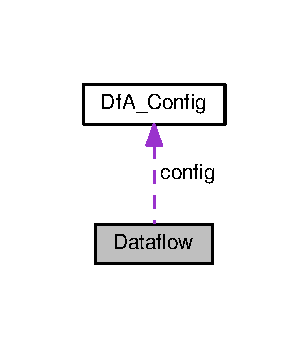
\includegraphics[width=148pt]{classDataflow__coll__graph}
\end{center}
\end{figure}
\subsection*{Public Member Functions}
\begin{DoxyCompactItemize}
\item 
\hyperlink{classDataflow_afebeeacfc0c5fdee45155ebb76dc62c8}{Dataflow} (string \hyperlink{classDataflow_a45d9ba19359e42a9a8d1fa089c994b17}{tag}, string hostname=dfa\+\_\+hostname, int port=dfa\+\_\+port)
\item 
void \hyperlink{classDataflow_a91f7c9eaf26223ff4c1da5f34fedb7be}{save} ()
\item 
\hyperlink{classTransformation}{Transformation} \& \hyperlink{classDataflow_ad0ad633cf3e23c76847e75ae388d29ea}{add\+\_\+transformation} (string \hyperlink{classDataflow_a45d9ba19359e42a9a8d1fa089c994b17}{tag}, vector$<$ \hyperlink{classSet}{Set} $>$ input\+\_\+sets, vector$<$ \hyperlink{classSet}{Set} $>$ output\+\_\+sets)
\item 
\hyperlink{classTransformation}{Transformation} \& \hyperlink{classDataflow_aad2e47f28cfdef9db53520328b88537a}{add\+\_\+transformation} (string \hyperlink{classDataflow_a45d9ba19359e42a9a8d1fa089c994b17}{tag}, \hyperlink{classSet}{Set} input\+\_\+set, \hyperlink{classSet}{Set} output\+\_\+set)
\item 
\hyperlink{classTransformation}{Transformation} \& \hyperlink{classDataflow_a36fad179e5f47f9a9ba1a598650c9b59}{add\+\_\+transformation} (string \hyperlink{classDataflow_a45d9ba19359e42a9a8d1fa089c994b17}{tag}, vector$<$ \hyperlink{classSet}{Set} $>$ input\+\_\+sets, \hyperlink{classSet}{Set} output\+\_\+set)
\item 
\hyperlink{classTransformation}{Transformation} \& \hyperlink{classDataflow_a777634e410ccfe677bf326858efd406f}{add\+\_\+transformation} (string \hyperlink{classDataflow_a45d9ba19359e42a9a8d1fa089c994b17}{tag}, \hyperlink{classSet}{Set} input\+\_\+set, vector$<$ \hyperlink{classSet}{Set} $>$ output\+\_\+sets)
\item 
\hyperlink{classSet}{Set} \& \hyperlink{classDataflow_a1b30ee20329211e193b90e8f8f78242f}{add\+\_\+set} (string \hyperlink{classDataflow_a45d9ba19359e42a9a8d1fa089c994b17}{tag})
\item 
\hyperlink{classSet}{Set} \& \hyperlink{classDataflow_abae00eba6d2eda469cba2391bd293915}{add\+\_\+set} (string \hyperlink{classDataflow_a45d9ba19359e42a9a8d1fa089c994b17}{tag}, string attribute\+\_\+name, attribute\+\_\+type attribute\+\_\+type)
\item 
\hyperlink{classSet}{Set} \& \hyperlink{classDataflow_a8621d2a61fbc9ec4ce8b21662d5804b9}{add\+\_\+set} (string \hyperlink{classDataflow_a45d9ba19359e42a9a8d1fa089c994b17}{tag}, vector$<$ string $>$ attribute\+\_\+names, vector$<$ attribute\+\_\+type $>$ attribute\+\_\+types)
\item 
string \hyperlink{classDataflow_a0d4fcfeba2d4fe22283c925d22eca17d}{get\+\_\+tag} ()
\item 
string \hyperlink{classDataflow_aa1023af477da09f5dcb63b048e19692e}{get\+\_\+specification} ()
\item 
vector$<$ \hyperlink{classTransformation}{Transformation} $>$ \hyperlink{classDataflow_a947b0d9382901eb90277f648b40f6946}{get\+\_\+sorted\+\_\+transformations} ()
\item 
int \hyperlink{classDataflow_af25c9cda8407c89e7099d680270e1a38}{get\+\_\+dependent\+\_\+transformation\+\_\+position\+\_\+from\+\_\+dataset\+\_\+tag} (vector$<$ \hyperlink{classTransformation}{Transformation} $>$ vec\+\_\+transformations, int current\+\_\+transformation\+\_\+position, vector$<$ string $>$ dataset\+\_\+tags)
\end{DoxyCompactItemize}
\subsection*{Protected Member Functions}
\begin{DoxyCompactItemize}
\item 
string \hyperlink{classDataflow_ace58f5775ef9eb6fb155d9280c5f2842}{get\+\_\+post\+\_\+message} ()
\end{DoxyCompactItemize}
\subsection*{Protected Attributes}
\begin{DoxyCompactItemize}
\item 
\mbox{\Hypertarget{classDataflow_a9194612ab9663190100ac63ef4a570ca}\label{classDataflow_a9194612ab9663190100ac63ef4a570ca}} 
\hyperlink{structDfA__Config}{Df\+A\+\_\+\+Config} \hyperlink{classDataflow_a9194612ab9663190100ac63ef4a570ca}{config}
\begin{DoxyCompactList}\small\item\em dataflow configuration \end{DoxyCompactList}\item 
\mbox{\Hypertarget{classDataflow_a45d9ba19359e42a9a8d1fa089c994b17}\label{classDataflow_a45d9ba19359e42a9a8d1fa089c994b17}} 
string \hyperlink{classDataflow_a45d9ba19359e42a9a8d1fa089c994b17}{tag}
\begin{DoxyCompactList}\small\item\em dataflow tag \end{DoxyCompactList}\item 
\mbox{\Hypertarget{classDataflow_a8b7aa91c6867e58d0829f2fdf0f74012}\label{classDataflow_a8b7aa91c6867e58d0829f2fdf0f74012}} 
map$<$ string, \hyperlink{classTransformation}{Transformation} $>$ \hyperlink{classDataflow_a8b7aa91c6867e58d0829f2fdf0f74012}{transformations}
\begin{DoxyCompactList}\small\item\em set of data transformations \end{DoxyCompactList}\item 
\mbox{\Hypertarget{classDataflow_a9adaff2ceea3186eb28aebf42b5c6911}\label{classDataflow_a9adaff2ceea3186eb28aebf42b5c6911}} 
map$<$ string, \hyperlink{classSet}{Set} $>$ \hyperlink{classDataflow_a9adaff2ceea3186eb28aebf42b5c6911}{sets}
\begin{DoxyCompactList}\small\item\em set of datasets \end{DoxyCompactList}\end{DoxyCompactItemize}


\subsection{Detailed Description}
Class to represent a dataflow specification (prospective provenance). 

\subsection{Constructor \& Destructor Documentation}
\mbox{\Hypertarget{classDataflow_afebeeacfc0c5fdee45155ebb76dc62c8}\label{classDataflow_afebeeacfc0c5fdee45155ebb76dc62c8}} 
\index{Dataflow@{Dataflow}!Dataflow@{Dataflow}}
\index{Dataflow@{Dataflow}!Dataflow@{Dataflow}}
\subsubsection{\texorpdfstring{Dataflow()}{Dataflow()}}
{\footnotesize\ttfamily Dataflow\+::\+Dataflow (\begin{DoxyParamCaption}\item[{string}]{tag,  }\item[{string}]{hostname = {\ttfamily dfa\+\_\+hostname},  }\item[{int}]{port = {\ttfamily dfa\+\_\+port} }\end{DoxyParamCaption})\hspace{0.3cm}{\ttfamily [inline]}}

Constructor of a dataflow specification 
\begin{DoxyParams}{Parameters}
{\em tag} & a dataflow tag \\
\hline
{\em hostname} & an optional argument that corresponds to the hostname of Df\+Analyzer R\+E\+S\+Tful server \\
\hline
{\em port} & an optional argument that corresponds to the port of Df\+Analyzer R\+E\+S\+Tful server. \\
\hline
\end{DoxyParams}


\subsection{Member Function Documentation}
\mbox{\Hypertarget{classDataflow_a1b30ee20329211e193b90e8f8f78242f}\label{classDataflow_a1b30ee20329211e193b90e8f8f78242f}} 
\index{Dataflow@{Dataflow}!add\+\_\+set@{add\+\_\+set}}
\index{add\+\_\+set@{add\+\_\+set}!Dataflow@{Dataflow}}
\subsubsection{\texorpdfstring{add\+\_\+set()}{add\_set()}\hspace{0.1cm}{\footnotesize\ttfamily [1/3]}}
{\footnotesize\ttfamily \hyperlink{classSet}{Set} \& Dataflow\+::add\+\_\+set (\begin{DoxyParamCaption}\item[{string}]{tag }\end{DoxyParamCaption})}

Add a dataset to the dataflow specification. 
\begin{DoxyParams}{Parameters}
{\em tag} & a dataset tag \\
\hline
\end{DoxyParams}
\mbox{\Hypertarget{classDataflow_abae00eba6d2eda469cba2391bd293915}\label{classDataflow_abae00eba6d2eda469cba2391bd293915}} 
\index{Dataflow@{Dataflow}!add\+\_\+set@{add\+\_\+set}}
\index{add\+\_\+set@{add\+\_\+set}!Dataflow@{Dataflow}}
\subsubsection{\texorpdfstring{add\+\_\+set()}{add\_set()}\hspace{0.1cm}{\footnotesize\ttfamily [2/3]}}
{\footnotesize\ttfamily \hyperlink{classSet}{Set} \& Dataflow\+::add\+\_\+set (\begin{DoxyParamCaption}\item[{string}]{tag,  }\item[{string}]{attribute\+\_\+name,  }\item[{attribute\+\_\+type}]{attribute\+\_\+type }\end{DoxyParamCaption})}

Add a dataset to the dataflow specification. 
\begin{DoxyParams}{Parameters}
{\em tag} & a dataset tag \\
\hline
{\em attribute\+\_\+name} & an attribute name \\
\hline
{\em attribute\+\_\+type} & an attribute types \\
\hline
\end{DoxyParams}
\mbox{\Hypertarget{classDataflow_a8621d2a61fbc9ec4ce8b21662d5804b9}\label{classDataflow_a8621d2a61fbc9ec4ce8b21662d5804b9}} 
\index{Dataflow@{Dataflow}!add\+\_\+set@{add\+\_\+set}}
\index{add\+\_\+set@{add\+\_\+set}!Dataflow@{Dataflow}}
\subsubsection{\texorpdfstring{add\+\_\+set()}{add\_set()}\hspace{0.1cm}{\footnotesize\ttfamily [3/3]}}
{\footnotesize\ttfamily \hyperlink{classSet}{Set} \& Dataflow\+::add\+\_\+set (\begin{DoxyParamCaption}\item[{string}]{tag,  }\item[{vector$<$ string $>$}]{attribute\+\_\+names,  }\item[{vector$<$ attribute\+\_\+type $>$}]{attribute\+\_\+types }\end{DoxyParamCaption})}

Add a dataset to the dataflow specification. 
\begin{DoxyParams}{Parameters}
{\em tag} & a dataset tag \\
\hline
{\em attribute\+\_\+names} & a set of attribute names \\
\hline
{\em attribute\+\_\+types} & a set of attribute types \\
\hline
\end{DoxyParams}
\mbox{\Hypertarget{classDataflow_ad0ad633cf3e23c76847e75ae388d29ea}\label{classDataflow_ad0ad633cf3e23c76847e75ae388d29ea}} 
\index{Dataflow@{Dataflow}!add\+\_\+transformation@{add\+\_\+transformation}}
\index{add\+\_\+transformation@{add\+\_\+transformation}!Dataflow@{Dataflow}}
\subsubsection{\texorpdfstring{add\+\_\+transformation()}{add\_transformation()}\hspace{0.1cm}{\footnotesize\ttfamily [1/4]}}
{\footnotesize\ttfamily \hyperlink{classTransformation}{Transformation} \& Dataflow\+::add\+\_\+transformation (\begin{DoxyParamCaption}\item[{string}]{tag,  }\item[{vector$<$ \hyperlink{classSet}{Set} $>$}]{input\+\_\+sets,  }\item[{vector$<$ \hyperlink{classSet}{Set} $>$}]{output\+\_\+sets }\end{DoxyParamCaption})}

Add a data transformation to the dataflow specification. 
\begin{DoxyParams}{Parameters}
{\em tag} & a dataflow tag \\
\hline
{\em input\+\_\+sets} & a set of input datasets \\
\hline
{\em output\+\_\+sets} & a set of output datasets \\
\hline
\end{DoxyParams}
\mbox{\Hypertarget{classDataflow_aad2e47f28cfdef9db53520328b88537a}\label{classDataflow_aad2e47f28cfdef9db53520328b88537a}} 
\index{Dataflow@{Dataflow}!add\+\_\+transformation@{add\+\_\+transformation}}
\index{add\+\_\+transformation@{add\+\_\+transformation}!Dataflow@{Dataflow}}
\subsubsection{\texorpdfstring{add\+\_\+transformation()}{add\_transformation()}\hspace{0.1cm}{\footnotesize\ttfamily [2/4]}}
{\footnotesize\ttfamily \hyperlink{classTransformation}{Transformation} \& Dataflow\+::add\+\_\+transformation (\begin{DoxyParamCaption}\item[{string}]{tag,  }\item[{\hyperlink{classSet}{Set}}]{input\+\_\+set,  }\item[{\hyperlink{classSet}{Set}}]{output\+\_\+set }\end{DoxyParamCaption})}

Add a data transformation to the dataflow specification. 
\begin{DoxyParams}{Parameters}
{\em tag} & a dataflow tag \\
\hline
{\em input\+\_\+set} & an input dataset \\
\hline
{\em output\+\_\+set} & an output dataset \\
\hline
\end{DoxyParams}
\mbox{\Hypertarget{classDataflow_a36fad179e5f47f9a9ba1a598650c9b59}\label{classDataflow_a36fad179e5f47f9a9ba1a598650c9b59}} 
\index{Dataflow@{Dataflow}!add\+\_\+transformation@{add\+\_\+transformation}}
\index{add\+\_\+transformation@{add\+\_\+transformation}!Dataflow@{Dataflow}}
\subsubsection{\texorpdfstring{add\+\_\+transformation()}{add\_transformation()}\hspace{0.1cm}{\footnotesize\ttfamily [3/4]}}
{\footnotesize\ttfamily \hyperlink{classTransformation}{Transformation} \& Dataflow\+::add\+\_\+transformation (\begin{DoxyParamCaption}\item[{string}]{tag,  }\item[{vector$<$ \hyperlink{classSet}{Set} $>$}]{input\+\_\+sets,  }\item[{\hyperlink{classSet}{Set}}]{output\+\_\+set }\end{DoxyParamCaption})}

Add a data transformation to the dataflow specification. 
\begin{DoxyParams}{Parameters}
{\em tag} & a dataflow tag \\
\hline
{\em input\+\_\+sets} & a set of input datasets \\
\hline
{\em output\+\_\+set} & an output dataset \\
\hline
\end{DoxyParams}
\mbox{\Hypertarget{classDataflow_a777634e410ccfe677bf326858efd406f}\label{classDataflow_a777634e410ccfe677bf326858efd406f}} 
\index{Dataflow@{Dataflow}!add\+\_\+transformation@{add\+\_\+transformation}}
\index{add\+\_\+transformation@{add\+\_\+transformation}!Dataflow@{Dataflow}}
\subsubsection{\texorpdfstring{add\+\_\+transformation()}{add\_transformation()}\hspace{0.1cm}{\footnotesize\ttfamily [4/4]}}
{\footnotesize\ttfamily \hyperlink{classTransformation}{Transformation} \& Dataflow\+::add\+\_\+transformation (\begin{DoxyParamCaption}\item[{string}]{tag,  }\item[{\hyperlink{classSet}{Set}}]{input\+\_\+set,  }\item[{vector$<$ \hyperlink{classSet}{Set} $>$}]{output\+\_\+sets }\end{DoxyParamCaption})}

Add a data transformation to the dataflow specification. 
\begin{DoxyParams}{Parameters}
{\em tag} & a dataflow tag \\
\hline
{\em input\+\_\+set} & an input dataset \\
\hline
{\em output\+\_\+sets} & a set of output datasets \\
\hline
\end{DoxyParams}
\mbox{\Hypertarget{classDataflow_af25c9cda8407c89e7099d680270e1a38}\label{classDataflow_af25c9cda8407c89e7099d680270e1a38}} 
\index{Dataflow@{Dataflow}!get\+\_\+dependent\+\_\+transformation\+\_\+position\+\_\+from\+\_\+dataset\+\_\+tag@{get\+\_\+dependent\+\_\+transformation\+\_\+position\+\_\+from\+\_\+dataset\+\_\+tag}}
\index{get\+\_\+dependent\+\_\+transformation\+\_\+position\+\_\+from\+\_\+dataset\+\_\+tag@{get\+\_\+dependent\+\_\+transformation\+\_\+position\+\_\+from\+\_\+dataset\+\_\+tag}!Dataflow@{Dataflow}}
\subsubsection{\texorpdfstring{get\+\_\+dependent\+\_\+transformation\+\_\+position\+\_\+from\+\_\+dataset\+\_\+tag()}{get\_dependent\_transformation\_position\_from\_dataset\_tag()}}
{\footnotesize\ttfamily int Dataflow\+::get\+\_\+dependent\+\_\+transformation\+\_\+position\+\_\+from\+\_\+dataset\+\_\+tag (\begin{DoxyParamCaption}\item[{vector$<$ \hyperlink{classTransformation}{Transformation} $>$}]{vec\+\_\+transformations,  }\item[{int}]{current\+\_\+transformation\+\_\+position,  }\item[{vector$<$ string $>$}]{dataset\+\_\+tags }\end{DoxyParamCaption})}

Get dependent data transformation position based on a dataset tag.  a set of data transformations  a data transformation position in vec\+\_\+transformations  a set of dataset tags to get their dependencies \begin{DoxyReturn}{Returns}
the position of the dependent data transformation 
\end{DoxyReturn}
\mbox{\Hypertarget{classDataflow_ace58f5775ef9eb6fb155d9280c5f2842}\label{classDataflow_ace58f5775ef9eb6fb155d9280c5f2842}} 
\index{Dataflow@{Dataflow}!get\+\_\+post\+\_\+message@{get\+\_\+post\+\_\+message}}
\index{get\+\_\+post\+\_\+message@{get\+\_\+post\+\_\+message}!Dataflow@{Dataflow}}
\subsubsection{\texorpdfstring{get\+\_\+post\+\_\+message()}{get\_post\_message()}}
{\footnotesize\ttfamily string Dataflow\+::get\+\_\+post\+\_\+message (\begin{DoxyParamCaption}{ }\end{DoxyParamCaption})\hspace{0.3cm}{\ttfamily [protected]}}

Get message to be sent to Df\+Analyzer server using an H\+T\+TP request with P\+O\+ST method. \begin{DoxyReturn}{Returns}
the message in H\+T\+TP request 
\end{DoxyReturn}
\mbox{\Hypertarget{classDataflow_a947b0d9382901eb90277f648b40f6946}\label{classDataflow_a947b0d9382901eb90277f648b40f6946}} 
\index{Dataflow@{Dataflow}!get\+\_\+sorted\+\_\+transformations@{get\+\_\+sorted\+\_\+transformations}}
\index{get\+\_\+sorted\+\_\+transformations@{get\+\_\+sorted\+\_\+transformations}!Dataflow@{Dataflow}}
\subsubsection{\texorpdfstring{get\+\_\+sorted\+\_\+transformations()}{get\_sorted\_transformations()}}
{\footnotesize\ttfamily vector$<$ \hyperlink{classTransformation}{Transformation} $>$ Dataflow\+::get\+\_\+sorted\+\_\+transformations (\begin{DoxyParamCaption}{ }\end{DoxyParamCaption})}

Get sorted data transformation. \begin{DoxyReturn}{Returns}
the set of sorted data transformations 
\end{DoxyReturn}
\mbox{\Hypertarget{classDataflow_aa1023af477da09f5dcb63b048e19692e}\label{classDataflow_aa1023af477da09f5dcb63b048e19692e}} 
\index{Dataflow@{Dataflow}!get\+\_\+specification@{get\+\_\+specification}}
\index{get\+\_\+specification@{get\+\_\+specification}!Dataflow@{Dataflow}}
\subsubsection{\texorpdfstring{get\+\_\+specification()}{get\_specification()}}
{\footnotesize\ttfamily string Dataflow\+::get\+\_\+specification (\begin{DoxyParamCaption}{ }\end{DoxyParamCaption})}

Get dataflow specification. \begin{DoxyReturn}{Returns}
the dataflow specification as a string 
\end{DoxyReturn}
\mbox{\Hypertarget{classDataflow_a0d4fcfeba2d4fe22283c925d22eca17d}\label{classDataflow_a0d4fcfeba2d4fe22283c925d22eca17d}} 
\index{Dataflow@{Dataflow}!get\+\_\+tag@{get\+\_\+tag}}
\index{get\+\_\+tag@{get\+\_\+tag}!Dataflow@{Dataflow}}
\subsubsection{\texorpdfstring{get\+\_\+tag()}{get\_tag()}}
{\footnotesize\ttfamily string Dataflow\+::get\+\_\+tag (\begin{DoxyParamCaption}{ }\end{DoxyParamCaption})}

Get dataflow tag \begin{DoxyReturn}{Returns}
the dataflow tag 
\end{DoxyReturn}
\mbox{\Hypertarget{classDataflow_a91f7c9eaf26223ff4c1da5f34fedb7be}\label{classDataflow_a91f7c9eaf26223ff4c1da5f34fedb7be}} 
\index{Dataflow@{Dataflow}!save@{save}}
\index{save@{save}!Dataflow@{Dataflow}}
\subsubsection{\texorpdfstring{save()}{save()}}
{\footnotesize\ttfamily void Dataflow\+::save (\begin{DoxyParamCaption}{ }\end{DoxyParamCaption})}

Save dataflow specification. 

The documentation for this class was generated from the following files\+:\begin{DoxyCompactItemize}
\item 
include/dataflow.\+h\item 
src/dataflow.\+cpp\end{DoxyCompactItemize}

\hypertarget{classDataset}{}\section{Dataset Class Reference}
\label{classDataset}\index{Dataset@{Dataset}}


{\ttfamily \#include $<$dataset.\+h$>$}

\subsection*{Public Member Functions}
\begin{DoxyCompactItemize}
\item 
\hyperlink{classDataset_a6eb00c4455a2d16ca5100996fd28ddf8}{Dataset} (string \hyperlink{classDataset_ae5a301fd4abf5979447bf16fc9775758}{tag})
\item 
void \hyperlink{classDataset_a86a705d9b163d64e812a085acbfb0a81}{add\+\_\+element\+\_\+with\+\_\+value} (string value)
\item 
void \hyperlink{classDataset_af945e29692f141411302850b29d55bfa}{add\+\_\+element\+\_\+with\+\_\+values} (vector$<$ string $>$ values)
\item 
void \hyperlink{classDataset_ac39864fdc124fe2893a42bbbd4a7ecc2}{clear\+\_\+elements} ()
\item 
string \hyperlink{classDataset_a6cb814dbc1aaa07d1a24d326de529302}{get\+\_\+tag} ()
\item 
vector$<$ \hyperlink{classElement}{Element} $>$ \& \hyperlink{classDataset_ad2048268e3dcbbcb8695daaadb00cc65}{get\+\_\+elements} ()
\item 
string \hyperlink{classDataset_a0d41185e47cb27299a46dec2d3717cb4}{get\+\_\+specification} ()
\end{DoxyCompactItemize}
\subsection*{Protected Attributes}
\begin{DoxyCompactItemize}
\item 
\mbox{\Hypertarget{classDataset_ae5a301fd4abf5979447bf16fc9775758}\label{classDataset_ae5a301fd4abf5979447bf16fc9775758}} 
string \hyperlink{classDataset_ae5a301fd4abf5979447bf16fc9775758}{tag}
\begin{DoxyCompactList}\small\item\em dataset tag \end{DoxyCompactList}\item 
\mbox{\Hypertarget{classDataset_a455ba8659783cb68146cb914a33f652b}\label{classDataset_a455ba8659783cb68146cb914a33f652b}} 
vector$<$ \hyperlink{classElement}{Element} $>$ \hyperlink{classDataset_a455ba8659783cb68146cb914a33f652b}{elements}
\begin{DoxyCompactList}\small\item\em set of data elements \end{DoxyCompactList}\end{DoxyCompactItemize}


\subsection{Detailed Description}
Class to represent a dataset (retrospective provenance). 

\subsection{Constructor \& Destructor Documentation}
\mbox{\Hypertarget{classDataset_a6eb00c4455a2d16ca5100996fd28ddf8}\label{classDataset_a6eb00c4455a2d16ca5100996fd28ddf8}} 
\index{Dataset@{Dataset}!Dataset@{Dataset}}
\index{Dataset@{Dataset}!Dataset@{Dataset}}
\subsubsection{\texorpdfstring{Dataset()}{Dataset()}}
{\footnotesize\ttfamily Dataset\+::\+Dataset (\begin{DoxyParamCaption}\item[{string}]{tag }\end{DoxyParamCaption})\hspace{0.3cm}{\ttfamily [inline]}}

Constructor of a dataset. 
\begin{DoxyParams}{Parameters}
{\em tag} & a dataset tag \\
\hline
\end{DoxyParams}


\subsection{Member Function Documentation}
\mbox{\Hypertarget{classDataset_a86a705d9b163d64e812a085acbfb0a81}\label{classDataset_a86a705d9b163d64e812a085acbfb0a81}} 
\index{Dataset@{Dataset}!add\+\_\+element\+\_\+with\+\_\+value@{add\+\_\+element\+\_\+with\+\_\+value}}
\index{add\+\_\+element\+\_\+with\+\_\+value@{add\+\_\+element\+\_\+with\+\_\+value}!Dataset@{Dataset}}
\subsubsection{\texorpdfstring{add\+\_\+element\+\_\+with\+\_\+value()}{add\_element\_with\_value()}}
{\footnotesize\ttfamily void Dataset\+::add\+\_\+element\+\_\+with\+\_\+value (\begin{DoxyParamCaption}\item[{string}]{value }\end{DoxyParamCaption})}

Add a data element with a single value to dataset. 
\begin{DoxyParams}{Parameters}
{\em value} & an attribute value \\
\hline
\end{DoxyParams}
\mbox{\Hypertarget{classDataset_af945e29692f141411302850b29d55bfa}\label{classDataset_af945e29692f141411302850b29d55bfa}} 
\index{Dataset@{Dataset}!add\+\_\+element\+\_\+with\+\_\+values@{add\+\_\+element\+\_\+with\+\_\+values}}
\index{add\+\_\+element\+\_\+with\+\_\+values@{add\+\_\+element\+\_\+with\+\_\+values}!Dataset@{Dataset}}
\subsubsection{\texorpdfstring{add\+\_\+element\+\_\+with\+\_\+values()}{add\_element\_with\_values()}}
{\footnotesize\ttfamily void Dataset\+::add\+\_\+element\+\_\+with\+\_\+values (\begin{DoxyParamCaption}\item[{vector$<$ string $>$}]{values }\end{DoxyParamCaption})}

Add a data element with multiple attribute values. 
\begin{DoxyParams}{Parameters}
{\em values} & set of attribute values \\
\hline
\end{DoxyParams}
\mbox{\Hypertarget{classDataset_ac39864fdc124fe2893a42bbbd4a7ecc2}\label{classDataset_ac39864fdc124fe2893a42bbbd4a7ecc2}} 
\index{Dataset@{Dataset}!clear\+\_\+elements@{clear\+\_\+elements}}
\index{clear\+\_\+elements@{clear\+\_\+elements}!Dataset@{Dataset}}
\subsubsection{\texorpdfstring{clear\+\_\+elements()}{clear\_elements()}}
{\footnotesize\ttfamily void Dataset\+::clear\+\_\+elements (\begin{DoxyParamCaption}{ }\end{DoxyParamCaption})}

Clear the set of data elements. \mbox{\Hypertarget{classDataset_ad2048268e3dcbbcb8695daaadb00cc65}\label{classDataset_ad2048268e3dcbbcb8695daaadb00cc65}} 
\index{Dataset@{Dataset}!get\+\_\+elements@{get\+\_\+elements}}
\index{get\+\_\+elements@{get\+\_\+elements}!Dataset@{Dataset}}
\subsubsection{\texorpdfstring{get\+\_\+elements()}{get\_elements()}}
{\footnotesize\ttfamily vector$<$ \hyperlink{classElement}{Element} $>$ \& Dataset\+::get\+\_\+elements (\begin{DoxyParamCaption}{ }\end{DoxyParamCaption})}

Get the data elements. \begin{DoxyReturn}{Returns}
the reference of the set of data elements 
\end{DoxyReturn}
\mbox{\Hypertarget{classDataset_a0d41185e47cb27299a46dec2d3717cb4}\label{classDataset_a0d41185e47cb27299a46dec2d3717cb4}} 
\index{Dataset@{Dataset}!get\+\_\+specification@{get\+\_\+specification}}
\index{get\+\_\+specification@{get\+\_\+specification}!Dataset@{Dataset}}
\subsubsection{\texorpdfstring{get\+\_\+specification()}{get\_specification()}}
{\footnotesize\ttfamily string Dataset\+::get\+\_\+specification (\begin{DoxyParamCaption}{ }\end{DoxyParamCaption})}

Get dataset specification. \begin{DoxyReturn}{Returns}
the dataset specification 
\end{DoxyReturn}
\mbox{\Hypertarget{classDataset_a6cb814dbc1aaa07d1a24d326de529302}\label{classDataset_a6cb814dbc1aaa07d1a24d326de529302}} 
\index{Dataset@{Dataset}!get\+\_\+tag@{get\+\_\+tag}}
\index{get\+\_\+tag@{get\+\_\+tag}!Dataset@{Dataset}}
\subsubsection{\texorpdfstring{get\+\_\+tag()}{get\_tag()}}
{\footnotesize\ttfamily string Dataset\+::get\+\_\+tag (\begin{DoxyParamCaption}{ }\end{DoxyParamCaption})}

Get the dataset tag. \begin{DoxyReturn}{Returns}
the dataset tag 
\end{DoxyReturn}


The documentation for this class was generated from the following files\+:\begin{DoxyCompactItemize}
\item 
include/dataset.\+h\item 
src/dataset.\+cpp\end{DoxyCompactItemize}

\hypertarget{classDependency}{}\section{Dependency Class Reference}
\label{classDependency}\index{Dependency@{Dependency}}


{\ttfamily \#include $<$dependency.\+h$>$}

\subsection*{Public Member Functions}
\begin{DoxyCompactItemize}
\item 
\hyperlink{classDependency_aa92957076c5000d1d3a56073302f1a41}{Dependency} ()
\item 
void \hyperlink{classDependency_a2436d5c4e0363832d2f81163467de426}{add\+\_\+transformation\+\_\+tag} (string transformation\+\_\+tag)
\item 
void \hyperlink{classDependency_aba3c43b4eb1e2429143cf297122f92ef}{add\+\_\+transformation\+\_\+ids} (vector$<$ int $>$ \hyperlink{classDependency_a357743c29d1e50ea6a06f0d89e4fa58c}{transformation\+\_\+ids})
\item 
void \hyperlink{classDependency_ac942f51b05df8875957b99ce74b9baec}{set\+\_\+transformation\+\_\+tags} (vector$<$ string $>$ \hyperlink{classDependency_a080b8391c054aaf43a7a6dfa9d57e125}{transformation\+\_\+tags})
\item 
vector$<$ string $>$ \& \hyperlink{classDependency_a89bbac105889b8fcf84a32f731a3a0b8}{get\+\_\+transformation\+\_\+tags} ()
\item 
vector$<$ vector$<$ int $>$ $>$ \& \hyperlink{classDependency_a9854eb2da947e302cefa36d25a880208}{get\+\_\+transformation\+\_\+ids} ()
\item 
string \hyperlink{classDependency_a158cbadc3e5d8a2a062a0f70c130821f}{get\+\_\+transformation\+\_\+tags\+\_\+as\+\_\+string} ()
\item 
string \hyperlink{classDependency_ab83b7f76991bb3f0ae6a42631002c8f4}{get\+\_\+transformation\+\_\+ids\+\_\+as\+\_\+string} ()
\item 
string \hyperlink{classDependency_adbff6153e89ab5a4143ee4f139a6f43a}{get\+\_\+specification} ()
\end{DoxyCompactItemize}
\subsection*{Protected Attributes}
\begin{DoxyCompactItemize}
\item 
\mbox{\Hypertarget{classDependency_a080b8391c054aaf43a7a6dfa9d57e125}\label{classDependency_a080b8391c054aaf43a7a6dfa9d57e125}} 
vector$<$ string $>$ \hyperlink{classDependency_a080b8391c054aaf43a7a6dfa9d57e125}{transformation\+\_\+tags}
\begin{DoxyCompactList}\small\item\em set of dependent data transformations \end{DoxyCompactList}\item 
\mbox{\Hypertarget{classDependency_a357743c29d1e50ea6a06f0d89e4fa58c}\label{classDependency_a357743c29d1e50ea6a06f0d89e4fa58c}} 
vector$<$ vector$<$ int $>$ $>$ \hyperlink{classDependency_a357743c29d1e50ea6a06f0d89e4fa58c}{transformation\+\_\+ids}
\begin{DoxyCompactList}\small\item\em set of tasks identifiers to the dependent data transformations \end{DoxyCompactList}\end{DoxyCompactItemize}


\subsection{Detailed Description}
Class to represent a data dependency (retrospective provenance). 

\subsection{Constructor \& Destructor Documentation}
\mbox{\Hypertarget{classDependency_aa92957076c5000d1d3a56073302f1a41}\label{classDependency_aa92957076c5000d1d3a56073302f1a41}} 
\index{Dependency@{Dependency}!Dependency@{Dependency}}
\index{Dependency@{Dependency}!Dependency@{Dependency}}
\subsubsection{\texorpdfstring{Dependency()}{Dependency()}}
{\footnotesize\ttfamily Dependency\+::\+Dependency (\begin{DoxyParamCaption}{ }\end{DoxyParamCaption})\hspace{0.3cm}{\ttfamily [inline]}}

Constructor of a data dependency. 

\subsection{Member Function Documentation}
\mbox{\Hypertarget{classDependency_aba3c43b4eb1e2429143cf297122f92ef}\label{classDependency_aba3c43b4eb1e2429143cf297122f92ef}} 
\index{Dependency@{Dependency}!add\+\_\+transformation\+\_\+ids@{add\+\_\+transformation\+\_\+ids}}
\index{add\+\_\+transformation\+\_\+ids@{add\+\_\+transformation\+\_\+ids}!Dependency@{Dependency}}
\subsubsection{\texorpdfstring{add\+\_\+transformation\+\_\+ids()}{add\_transformation\_ids()}}
{\footnotesize\ttfamily void Dependency\+::add\+\_\+transformation\+\_\+ids (\begin{DoxyParamCaption}\item[{vector$<$ int $>$}]{transformation\+\_\+ids }\end{DoxyParamCaption})}

Add task identifiers to the set of task identifiers. 
\begin{DoxyParams}{Parameters}
{\em transformation\+\_\+ids} & a set of data transformation identifiers \\
\hline
\end{DoxyParams}
\mbox{\Hypertarget{classDependency_a2436d5c4e0363832d2f81163467de426}\label{classDependency_a2436d5c4e0363832d2f81163467de426}} 
\index{Dependency@{Dependency}!add\+\_\+transformation\+\_\+tag@{add\+\_\+transformation\+\_\+tag}}
\index{add\+\_\+transformation\+\_\+tag@{add\+\_\+transformation\+\_\+tag}!Dependency@{Dependency}}
\subsubsection{\texorpdfstring{add\+\_\+transformation\+\_\+tag()}{add\_transformation\_tag()}}
{\footnotesize\ttfamily void Dependency\+::add\+\_\+transformation\+\_\+tag (\begin{DoxyParamCaption}\item[{string}]{transformation\+\_\+tag }\end{DoxyParamCaption})}

Add a data transformation tag. 
\begin{DoxyParams}{Parameters}
{\em transformation\+\_\+tag} & a data transformation tag \\
\hline
\end{DoxyParams}
\mbox{\Hypertarget{classDependency_adbff6153e89ab5a4143ee4f139a6f43a}\label{classDependency_adbff6153e89ab5a4143ee4f139a6f43a}} 
\index{Dependency@{Dependency}!get\+\_\+specification@{get\+\_\+specification}}
\index{get\+\_\+specification@{get\+\_\+specification}!Dependency@{Dependency}}
\subsubsection{\texorpdfstring{get\+\_\+specification()}{get\_specification()}}
{\footnotesize\ttfamily string Dependency\+::get\+\_\+specification (\begin{DoxyParamCaption}{ }\end{DoxyParamCaption})}

Get data dependency specification. \begin{DoxyReturn}{Returns}
the data dependency specification 
\end{DoxyReturn}
\mbox{\Hypertarget{classDependency_a9854eb2da947e302cefa36d25a880208}\label{classDependency_a9854eb2da947e302cefa36d25a880208}} 
\index{Dependency@{Dependency}!get\+\_\+transformation\+\_\+ids@{get\+\_\+transformation\+\_\+ids}}
\index{get\+\_\+transformation\+\_\+ids@{get\+\_\+transformation\+\_\+ids}!Dependency@{Dependency}}
\subsubsection{\texorpdfstring{get\+\_\+transformation\+\_\+ids()}{get\_transformation\_ids()}}
{\footnotesize\ttfamily vector$<$ vector$<$ int $>$ $>$ \& Dependency\+::get\+\_\+transformation\+\_\+ids (\begin{DoxyParamCaption}{ }\end{DoxyParamCaption})}

Get the tasks identifiers to the dependent data transformations. \begin{DoxyReturn}{Returns}
the reference of the set of task identifiers 
\end{DoxyReturn}
\mbox{\Hypertarget{classDependency_ab83b7f76991bb3f0ae6a42631002c8f4}\label{classDependency_ab83b7f76991bb3f0ae6a42631002c8f4}} 
\index{Dependency@{Dependency}!get\+\_\+transformation\+\_\+ids\+\_\+as\+\_\+string@{get\+\_\+transformation\+\_\+ids\+\_\+as\+\_\+string}}
\index{get\+\_\+transformation\+\_\+ids\+\_\+as\+\_\+string@{get\+\_\+transformation\+\_\+ids\+\_\+as\+\_\+string}!Dependency@{Dependency}}
\subsubsection{\texorpdfstring{get\+\_\+transformation\+\_\+ids\+\_\+as\+\_\+string()}{get\_transformation\_ids\_as\_string()}}
{\footnotesize\ttfamily string Dependency\+::get\+\_\+transformation\+\_\+ids\+\_\+as\+\_\+string (\begin{DoxyParamCaption}{ }\end{DoxyParamCaption})}

Get the task identifiers to the dependent data transformation. \begin{DoxyReturn}{Returns}
the set of task identifiers as a string 
\end{DoxyReturn}
\mbox{\Hypertarget{classDependency_a89bbac105889b8fcf84a32f731a3a0b8}\label{classDependency_a89bbac105889b8fcf84a32f731a3a0b8}} 
\index{Dependency@{Dependency}!get\+\_\+transformation\+\_\+tags@{get\+\_\+transformation\+\_\+tags}}
\index{get\+\_\+transformation\+\_\+tags@{get\+\_\+transformation\+\_\+tags}!Dependency@{Dependency}}
\subsubsection{\texorpdfstring{get\+\_\+transformation\+\_\+tags()}{get\_transformation\_tags()}}
{\footnotesize\ttfamily vector$<$ string $>$ \& Dependency\+::get\+\_\+transformation\+\_\+tags (\begin{DoxyParamCaption}{ }\end{DoxyParamCaption})}

Get the data transformation tags. \begin{DoxyReturn}{Returns}
the reference of the set of data transformation tags 
\end{DoxyReturn}
\mbox{\Hypertarget{classDependency_a158cbadc3e5d8a2a062a0f70c130821f}\label{classDependency_a158cbadc3e5d8a2a062a0f70c130821f}} 
\index{Dependency@{Dependency}!get\+\_\+transformation\+\_\+tags\+\_\+as\+\_\+string@{get\+\_\+transformation\+\_\+tags\+\_\+as\+\_\+string}}
\index{get\+\_\+transformation\+\_\+tags\+\_\+as\+\_\+string@{get\+\_\+transformation\+\_\+tags\+\_\+as\+\_\+string}!Dependency@{Dependency}}
\subsubsection{\texorpdfstring{get\+\_\+transformation\+\_\+tags\+\_\+as\+\_\+string()}{get\_transformation\_tags\_as\_string()}}
{\footnotesize\ttfamily string Dependency\+::get\+\_\+transformation\+\_\+tags\+\_\+as\+\_\+string (\begin{DoxyParamCaption}{ }\end{DoxyParamCaption})}

Get the data transformation tags. \begin{DoxyReturn}{Returns}
the data transformation tags as a string 
\end{DoxyReturn}
\mbox{\Hypertarget{classDependency_ac942f51b05df8875957b99ce74b9baec}\label{classDependency_ac942f51b05df8875957b99ce74b9baec}} 
\index{Dependency@{Dependency}!set\+\_\+transformation\+\_\+tags@{set\+\_\+transformation\+\_\+tags}}
\index{set\+\_\+transformation\+\_\+tags@{set\+\_\+transformation\+\_\+tags}!Dependency@{Dependency}}
\subsubsection{\texorpdfstring{set\+\_\+transformation\+\_\+tags()}{set\_transformation\_tags()}}
{\footnotesize\ttfamily void Dependency\+::set\+\_\+transformation\+\_\+tags (\begin{DoxyParamCaption}\item[{vector$<$ string $>$}]{transformation\+\_\+tags }\end{DoxyParamCaption})}

\hyperlink{classSet}{Set} a set of data transformation tags. 
\begin{DoxyParams}{Parameters}
{\em transformation\+\_\+tags} & a set of data transformation\+\_\+tags \\
\hline
\end{DoxyParams}


The documentation for this class was generated from the following files\+:\begin{DoxyCompactItemize}
\item 
include/dependency.\+h\item 
src/dependency.\+cpp\end{DoxyCompactItemize}

\hypertarget{structDfA__Config}{}\section{Df\+A\+\_\+\+Config Struct Reference}
\label{structDfA__Config}\index{Df\+A\+\_\+\+Config@{Df\+A\+\_\+\+Config}}
\subsection*{Public Attributes}
\begin{DoxyCompactItemize}
\item 
\mbox{\Hypertarget{structDfA__Config_a8b2084e26f2d851c1dc7830cfb833cae}\label{structDfA__Config_a8b2084e26f2d851c1dc7830cfb833cae}} 
string \hyperlink{structDfA__Config_a8b2084e26f2d851c1dc7830cfb833cae}{hostname}
\begin{DoxyCompactList}\small\item\em hostname of dfanalyzer server \end{DoxyCompactList}\item 
\mbox{\Hypertarget{structDfA__Config_a9da44f82fe807f72b43f96f548f24b1c}\label{structDfA__Config_a9da44f82fe807f72b43f96f548f24b1c}} 
int \hyperlink{structDfA__Config_a9da44f82fe807f72b43f96f548f24b1c}{port}
\begin{DoxyCompactList}\small\item\em port of dfanalyzer server \end{DoxyCompactList}\end{DoxyCompactItemize}


The documentation for this struct was generated from the following file\+:\begin{DoxyCompactItemize}
\item 
include/dfa\+\_\+configuration\+\_\+struct.\+h\end{DoxyCompactItemize}

\hypertarget{classElement}{}\section{Element Class Reference}
\label{classElement}\index{Element@{Element}}


{\ttfamily \#include $<$element.\+h$>$}

\subsection*{Public Member Functions}
\begin{DoxyCompactItemize}
\item 
\hyperlink{classElement_ab0d0e20be9a36ae676202db753faeec9}{Element} ()
\item 
\hyperlink{classElement_ac5749aba608dc8bfb68c7e996d159cb7}{Element} (string value)
\item 
\hyperlink{classElement_a628516fcaf54458e35ffbcb3a9082e99}{Element} (vector$<$ string $>$ \hyperlink{classElement_ae2b88bc22f391bc263521096c2613897}{values})
\item 
void \hyperlink{classElement_a67439f02d44fb2fa834d9a7b223709a8}{add\+\_\+value} (string value)
\item 
void \hyperlink{classElement_aa962031ba982f58e7bd5caceb5b8d058}{set\+\_\+values} (vector$<$ string $>$ \hyperlink{classElement_ae2b88bc22f391bc263521096c2613897}{values})
\item 
vector$<$ string $>$ \& \hyperlink{classElement_ae1c0e14049aaa6b7a9c047039038de3a}{get\+\_\+values} ()
\item 
string \hyperlink{classElement_a50b58de922a1cb1ee1dea8abf789bb64}{get\+\_\+values\+\_\+as\+\_\+string} ()
\end{DoxyCompactItemize}
\subsection*{Protected Attributes}
\begin{DoxyCompactItemize}
\item 
\mbox{\Hypertarget{classElement_ae2b88bc22f391bc263521096c2613897}\label{classElement_ae2b88bc22f391bc263521096c2613897}} 
vector$<$ string $>$ \hyperlink{classElement_ae2b88bc22f391bc263521096c2613897}{values}
\begin{DoxyCompactList}\small\item\em set of attribute values \end{DoxyCompactList}\end{DoxyCompactItemize}


\subsection{Detailed Description}
Class to represent a data element (retrospective provenance). 

\subsection{Constructor \& Destructor Documentation}
\mbox{\Hypertarget{classElement_ab0d0e20be9a36ae676202db753faeec9}\label{classElement_ab0d0e20be9a36ae676202db753faeec9}} 
\index{Element@{Element}!Element@{Element}}
\index{Element@{Element}!Element@{Element}}
\subsubsection{\texorpdfstring{Element()}{Element()}\hspace{0.1cm}{\footnotesize\ttfamily [1/3]}}
{\footnotesize\ttfamily Element\+::\+Element (\begin{DoxyParamCaption}{ }\end{DoxyParamCaption})\hspace{0.3cm}{\ttfamily [inline]}}

Constructor of a data element. \mbox{\Hypertarget{classElement_ac5749aba608dc8bfb68c7e996d159cb7}\label{classElement_ac5749aba608dc8bfb68c7e996d159cb7}} 
\index{Element@{Element}!Element@{Element}}
\index{Element@{Element}!Element@{Element}}
\subsubsection{\texorpdfstring{Element()}{Element()}\hspace{0.1cm}{\footnotesize\ttfamily [2/3]}}
{\footnotesize\ttfamily Element\+::\+Element (\begin{DoxyParamCaption}\item[{string}]{value }\end{DoxyParamCaption})\hspace{0.3cm}{\ttfamily [inline]}}

Constructor of a data element. 
\begin{DoxyParams}{Parameters}
{\em value} & a single attribute value \\
\hline
\end{DoxyParams}
\mbox{\Hypertarget{classElement_a628516fcaf54458e35ffbcb3a9082e99}\label{classElement_a628516fcaf54458e35ffbcb3a9082e99}} 
\index{Element@{Element}!Element@{Element}}
\index{Element@{Element}!Element@{Element}}
\subsubsection{\texorpdfstring{Element()}{Element()}\hspace{0.1cm}{\footnotesize\ttfamily [3/3]}}
{\footnotesize\ttfamily Element\+::\+Element (\begin{DoxyParamCaption}\item[{vector$<$ string $>$}]{values }\end{DoxyParamCaption})\hspace{0.3cm}{\ttfamily [inline]}}

Constructor of a data element. 
\begin{DoxyParams}{Parameters}
{\em values} & a set of attribute values \\
\hline
\end{DoxyParams}


\subsection{Member Function Documentation}
\mbox{\Hypertarget{classElement_a67439f02d44fb2fa834d9a7b223709a8}\label{classElement_a67439f02d44fb2fa834d9a7b223709a8}} 
\index{Element@{Element}!add\+\_\+value@{add\+\_\+value}}
\index{add\+\_\+value@{add\+\_\+value}!Element@{Element}}
\subsubsection{\texorpdfstring{add\+\_\+value()}{add\_value()}}
{\footnotesize\ttfamily void Element\+::add\+\_\+value (\begin{DoxyParamCaption}\item[{string}]{value }\end{DoxyParamCaption})}

Add attribute value to a data element in an ordered manner. Each invocation of this member function will add the attribute value at the end of the set of attribute values. 
\begin{DoxyParams}{Parameters}
{\em value} & attribute value \\
\hline
\end{DoxyParams}
\mbox{\Hypertarget{classElement_ae1c0e14049aaa6b7a9c047039038de3a}\label{classElement_ae1c0e14049aaa6b7a9c047039038de3a}} 
\index{Element@{Element}!get\+\_\+values@{get\+\_\+values}}
\index{get\+\_\+values@{get\+\_\+values}!Element@{Element}}
\subsubsection{\texorpdfstring{get\+\_\+values()}{get\_values()}}
{\footnotesize\ttfamily vector$<$ string $>$ \& Element\+::get\+\_\+values (\begin{DoxyParamCaption}{ }\end{DoxyParamCaption})}

Get attribute values \begin{DoxyReturn}{Returns}
the attribute values 
\end{DoxyReturn}
\mbox{\Hypertarget{classElement_a50b58de922a1cb1ee1dea8abf789bb64}\label{classElement_a50b58de922a1cb1ee1dea8abf789bb64}} 
\index{Element@{Element}!get\+\_\+values\+\_\+as\+\_\+string@{get\+\_\+values\+\_\+as\+\_\+string}}
\index{get\+\_\+values\+\_\+as\+\_\+string@{get\+\_\+values\+\_\+as\+\_\+string}!Element@{Element}}
\subsubsection{\texorpdfstring{get\+\_\+values\+\_\+as\+\_\+string()}{get\_values\_as\_string()}}
{\footnotesize\ttfamily string Element\+::get\+\_\+values\+\_\+as\+\_\+string (\begin{DoxyParamCaption}{ }\end{DoxyParamCaption})}

Get attribute values. \begin{DoxyReturn}{Returns}
the attribute values as string. 
\end{DoxyReturn}
\mbox{\Hypertarget{classElement_aa962031ba982f58e7bd5caceb5b8d058}\label{classElement_aa962031ba982f58e7bd5caceb5b8d058}} 
\index{Element@{Element}!set\+\_\+values@{set\+\_\+values}}
\index{set\+\_\+values@{set\+\_\+values}!Element@{Element}}
\subsubsection{\texorpdfstring{set\+\_\+values()}{set\_values()}}
{\footnotesize\ttfamily void Element\+::set\+\_\+values (\begin{DoxyParamCaption}\item[{vector$<$ string $>$}]{values }\end{DoxyParamCaption})}

\hyperlink{classSet}{Set} attribute values. 
\begin{DoxyParams}{Parameters}
{\em a} & set of attribute values \\
\hline
\end{DoxyParams}


The documentation for this class was generated from the following files\+:\begin{DoxyCompactItemize}
\item 
include/element.\+h\item 
src/element.\+cpp\end{DoxyCompactItemize}

\hypertarget{classExtractor}{}\section{Extractor Class Reference}
\label{classExtractor}\index{Extractor@{Extractor}}


{\ttfamily \#include $<$extractor.\+h$>$}

\subsection*{Public Member Functions}
\begin{DoxyCompactItemize}
\item 
\hyperlink{classExtractor_ab1bbe102a4f6087831d6090bb7096c09}{Extractor} (string \hyperlink{classExtractor_a53f998b8d2fb1032f6c86f0d04a2ffc8}{tag}, string \hyperlink{classExtractor_acafbe087b3bae5259d6e6c7bb7999255}{set\+\_\+tag}, method\+\_\+type \hyperlink{classExtractor_a9167bf123b2164a89175253d64bdab43}{method}, cartridge\+\_\+type \hyperlink{classExtractor_a19cea477abf042cec1ad70cb56bbd973}{cartridge})
\item 
void \hyperlink{classExtractor_ae82579657e380e26facb22dbf2c52966}{add\+\_\+attribute} (string name, attribute\+\_\+type type)
\item 
void \hyperlink{classExtractor_a429e9f3ad4cfeb712b01c2617f2253e6}{add\+\_\+attributes} (vector$<$ string $>$ names, vector$<$ attribute\+\_\+type $>$ types)
\item 
string \hyperlink{classExtractor_ad23a148dddb5a78557b84baa00829fc4}{get\+\_\+tag} ()
\item 
string \hyperlink{classExtractor_a133d1cd6a2749254614d7cebd9832cea}{get\+\_\+set\+\_\+tag} ()
\item 
\hyperlink{classAttribute}{Attribute} \& \hyperlink{classExtractor_a56a4af532b92d7dbe7aa6f9db242e992}{get\+\_\+attribute\+\_\+by\+\_\+name} (string name)
\item 
string \hyperlink{classExtractor_ae76e664785cb63537295ce404e728191}{get\+\_\+method} ()
\item 
string \hyperlink{classExtractor_a44ed7358715318d58dc5246ab43fcd2b}{get\+\_\+cartridge} ()
\item 
string \hyperlink{classExtractor_ad2576ada89be5c806e8f0cbc319e8f19}{get\+\_\+specification} ()
\end{DoxyCompactItemize}
\subsection*{Protected Attributes}
\begin{DoxyCompactItemize}
\item 
\mbox{\Hypertarget{classExtractor_a53f998b8d2fb1032f6c86f0d04a2ffc8}\label{classExtractor_a53f998b8d2fb1032f6c86f0d04a2ffc8}} 
string \hyperlink{classExtractor_a53f998b8d2fb1032f6c86f0d04a2ffc8}{tag}
\begin{DoxyCompactList}\small\item\em extractor tag \end{DoxyCompactList}\item 
\mbox{\Hypertarget{classExtractor_acafbe087b3bae5259d6e6c7bb7999255}\label{classExtractor_acafbe087b3bae5259d6e6c7bb7999255}} 
string \hyperlink{classExtractor_acafbe087b3bae5259d6e6c7bb7999255}{set\+\_\+tag}
\begin{DoxyCompactList}\small\item\em dataset tag which extracted data will be loaded \end{DoxyCompactList}\item 
\mbox{\Hypertarget{classExtractor_a9167bf123b2164a89175253d64bdab43}\label{classExtractor_a9167bf123b2164a89175253d64bdab43}} 
method\+\_\+type \hyperlink{classExtractor_a9167bf123b2164a89175253d64bdab43}{method}
\begin{DoxyCompactList}\small\item\em method of the raw data extractor, which can be E\+X\+T\+R\+A\+C\+T\+I\+ON or I\+N\+D\+E\+X\+I\+NG \end{DoxyCompactList}\item 
\mbox{\Hypertarget{classExtractor_a19cea477abf042cec1ad70cb56bbd973}\label{classExtractor_a19cea477abf042cec1ad70cb56bbd973}} 
cartridge\+\_\+type \hyperlink{classExtractor_a19cea477abf042cec1ad70cb56bbd973}{cartridge}
\begin{DoxyCompactList}\small\item\em cartridge of the raw data extractor, which can be C\+SV (extraction or indexing), P\+R\+O\+G\+R\+AM (extraction), F\+A\+S\+T\+B\+IT, O\+P\+T\+I\+M\+I\+Z\+E\+D\+\_\+\+F\+A\+S\+T\+B\+IT, P\+O\+S\+T\+G\+R\+E\+S\+\_\+\+R\+AW (indexing) \end{DoxyCompactList}\item 
\mbox{\Hypertarget{classExtractor_a16cd88e5932d56a8628af94df5af9cc4}\label{classExtractor_a16cd88e5932d56a8628af94df5af9cc4}} 
vector$<$ \hyperlink{classAttribute}{Attribute} $>$ \hyperlink{classExtractor_a16cd88e5932d56a8628af94df5af9cc4}{attributes}
\begin{DoxyCompactList}\small\item\em set of attributes \end{DoxyCompactList}\end{DoxyCompactItemize}


\subsection{Detailed Description}
Class to represent a data extractor specification (prospective provenance). 

\subsection{Constructor \& Destructor Documentation}
\mbox{\Hypertarget{classExtractor_ab1bbe102a4f6087831d6090bb7096c09}\label{classExtractor_ab1bbe102a4f6087831d6090bb7096c09}} 
\index{Extractor@{Extractor}!Extractor@{Extractor}}
\index{Extractor@{Extractor}!Extractor@{Extractor}}
\subsubsection{\texorpdfstring{Extractor()}{Extractor()}}
{\footnotesize\ttfamily Extractor\+::\+Extractor (\begin{DoxyParamCaption}\item[{string}]{tag,  }\item[{string}]{set\+\_\+tag,  }\item[{method\+\_\+type}]{method,  }\item[{cartridge\+\_\+type}]{cartridge }\end{DoxyParamCaption})\hspace{0.3cm}{\ttfamily [inline]}}

Constructor of a raw data extractor. 
\begin{DoxyParams}{Parameters}
{\em tag} & an extractor tag \\
\hline
{\em set\+\_\+tag} & a dataset tag \\
\hline
{\em method\+\_\+type} & an extraction or indexing method \\
\hline
{\em cartridge\+\_\+type} & a cartridge to be executed by the extractor \\
\hline
\end{DoxyParams}


\subsection{Member Function Documentation}
\mbox{\Hypertarget{classExtractor_ae82579657e380e26facb22dbf2c52966}\label{classExtractor_ae82579657e380e26facb22dbf2c52966}} 
\index{Extractor@{Extractor}!add\+\_\+attribute@{add\+\_\+attribute}}
\index{add\+\_\+attribute@{add\+\_\+attribute}!Extractor@{Extractor}}
\subsubsection{\texorpdfstring{add\+\_\+attribute()}{add\_attribute()}}
{\footnotesize\ttfamily void Extractor\+::add\+\_\+attribute (\begin{DoxyParamCaption}\item[{string}]{name,  }\item[{attribute\+\_\+type}]{type }\end{DoxyParamCaption})}

Add an attribute to be extracted. 
\begin{DoxyParams}{Parameters}
{\em name} & an attribute name \\
\hline
{\em type} & an attribute type \\
\hline
\end{DoxyParams}
\mbox{\Hypertarget{classExtractor_a429e9f3ad4cfeb712b01c2617f2253e6}\label{classExtractor_a429e9f3ad4cfeb712b01c2617f2253e6}} 
\index{Extractor@{Extractor}!add\+\_\+attributes@{add\+\_\+attributes}}
\index{add\+\_\+attributes@{add\+\_\+attributes}!Extractor@{Extractor}}
\subsubsection{\texorpdfstring{add\+\_\+attributes()}{add\_attributes()}}
{\footnotesize\ttfamily void Extractor\+::add\+\_\+attributes (\begin{DoxyParamCaption}\item[{vector$<$ string $>$}]{names,  }\item[{vector$<$ attribute\+\_\+type $>$}]{types }\end{DoxyParamCaption})}

Add a set of attributes 
\begin{DoxyParams}{Parameters}
{\em names} & a set of attribute names \\
\hline
{\em types} & a set of attribute types \\
\hline
\end{DoxyParams}
\mbox{\Hypertarget{classExtractor_a56a4af532b92d7dbe7aa6f9db242e992}\label{classExtractor_a56a4af532b92d7dbe7aa6f9db242e992}} 
\index{Extractor@{Extractor}!get\+\_\+attribute\+\_\+by\+\_\+name@{get\+\_\+attribute\+\_\+by\+\_\+name}}
\index{get\+\_\+attribute\+\_\+by\+\_\+name@{get\+\_\+attribute\+\_\+by\+\_\+name}!Extractor@{Extractor}}
\subsubsection{\texorpdfstring{get\+\_\+attribute\+\_\+by\+\_\+name()}{get\_attribute\_by\_name()}}
{\footnotesize\ttfamily \hyperlink{classAttribute}{Attribute} \& Extractor\+::get\+\_\+attribute\+\_\+by\+\_\+name (\begin{DoxyParamCaption}\item[{string}]{name }\end{DoxyParamCaption})}

Get the attribute given its name. 
\begin{DoxyParams}{Parameters}
{\em name} & an attribute name \\
\hline
\end{DoxyParams}
\begin{DoxyReturn}{Returns}
the reference of the attribute with the given name 
\end{DoxyReturn}
\mbox{\Hypertarget{classExtractor_a44ed7358715318d58dc5246ab43fcd2b}\label{classExtractor_a44ed7358715318d58dc5246ab43fcd2b}} 
\index{Extractor@{Extractor}!get\+\_\+cartridge@{get\+\_\+cartridge}}
\index{get\+\_\+cartridge@{get\+\_\+cartridge}!Extractor@{Extractor}}
\subsubsection{\texorpdfstring{get\+\_\+cartridge()}{get\_cartridge()}}
{\footnotesize\ttfamily string Extractor\+::get\+\_\+cartridge (\begin{DoxyParamCaption}{ }\end{DoxyParamCaption})}

Get the cartridge implemented by the raw data extractor. \begin{DoxyReturn}{Returns}
the extractor cartridge 
\end{DoxyReturn}
\mbox{\Hypertarget{classExtractor_ae76e664785cb63537295ce404e728191}\label{classExtractor_ae76e664785cb63537295ce404e728191}} 
\index{Extractor@{Extractor}!get\+\_\+method@{get\+\_\+method}}
\index{get\+\_\+method@{get\+\_\+method}!Extractor@{Extractor}}
\subsubsection{\texorpdfstring{get\+\_\+method()}{get\_method()}}
{\footnotesize\ttfamily string Extractor\+::get\+\_\+method (\begin{DoxyParamCaption}{ }\end{DoxyParamCaption})}

Get the method of raw data extractor. \begin{DoxyReturn}{Returns}
the extraction or indexing method 
\end{DoxyReturn}
\mbox{\Hypertarget{classExtractor_a133d1cd6a2749254614d7cebd9832cea}\label{classExtractor_a133d1cd6a2749254614d7cebd9832cea}} 
\index{Extractor@{Extractor}!get\+\_\+set\+\_\+tag@{get\+\_\+set\+\_\+tag}}
\index{get\+\_\+set\+\_\+tag@{get\+\_\+set\+\_\+tag}!Extractor@{Extractor}}
\subsubsection{\texorpdfstring{get\+\_\+set\+\_\+tag()}{get\_set\_tag()}}
{\footnotesize\ttfamily string Extractor\+::get\+\_\+set\+\_\+tag (\begin{DoxyParamCaption}{ }\end{DoxyParamCaption})}

Get the dataset tag. \begin{DoxyReturn}{Returns}
the dataset tag 
\end{DoxyReturn}
\mbox{\Hypertarget{classExtractor_ad2576ada89be5c806e8f0cbc319e8f19}\label{classExtractor_ad2576ada89be5c806e8f0cbc319e8f19}} 
\index{Extractor@{Extractor}!get\+\_\+specification@{get\+\_\+specification}}
\index{get\+\_\+specification@{get\+\_\+specification}!Extractor@{Extractor}}
\subsubsection{\texorpdfstring{get\+\_\+specification()}{get\_specification()}}
{\footnotesize\ttfamily string Extractor\+::get\+\_\+specification (\begin{DoxyParamCaption}{ }\end{DoxyParamCaption})}

Get the specification of raw data extractor. \begin{DoxyReturn}{Returns}
the extractor specification. 
\end{DoxyReturn}
\mbox{\Hypertarget{classExtractor_ad23a148dddb5a78557b84baa00829fc4}\label{classExtractor_ad23a148dddb5a78557b84baa00829fc4}} 
\index{Extractor@{Extractor}!get\+\_\+tag@{get\+\_\+tag}}
\index{get\+\_\+tag@{get\+\_\+tag}!Extractor@{Extractor}}
\subsubsection{\texorpdfstring{get\+\_\+tag()}{get\_tag()}}
{\footnotesize\ttfamily string Extractor\+::get\+\_\+tag (\begin{DoxyParamCaption}{ }\end{DoxyParamCaption})}

Get the raw data extractor tag. \begin{DoxyReturn}{Returns}
the extractor tag 
\end{DoxyReturn}


The documentation for this class was generated from the following files\+:\begin{DoxyCompactItemize}
\item 
include/extractor.\+h\item 
src/extractor.\+cpp\end{DoxyCompactItemize}

\hypertarget{classRawDataExtractor}{}\section{Raw\+Data\+Extractor Class Reference}
\label{classRawDataExtractor}\index{Raw\+Data\+Extractor@{Raw\+Data\+Extractor}}


{\ttfamily \#include $<$raw\+\_\+data\+\_\+extractor.\+h$>$}

\subsection*{Public Member Functions}
\begin{DoxyCompactItemize}
\item 
\hyperlink{classRawDataExtractor_a5152ed0ab55f6324964cd718572fcb31}{Raw\+Data\+Extractor} (string \hyperlink{classRawDataExtractor_a17902ee3cae7c15061ef208b11b0d300}{command\+\_\+line}, vector$<$ string $>$ \hyperlink{classRawDataExtractor_a23ce52343673f63a56c5c05cf15a3859}{attribute\+\_\+names}, vector$<$ attribute\+\_\+type $>$ \hyperlink{classRawDataExtractor_a0c5d6acb054f65891526b2fe1c5d1cf3}{attribute\+\_\+types})
\item 
void \hyperlink{classRawDataExtractor_aab89e89463d22ed6289f3193aa22ce59}{set\+\_\+attribute\+\_\+names} (vector$<$ string $>$ \hyperlink{classRawDataExtractor_a23ce52343673f63a56c5c05cf15a3859}{attribute\+\_\+names})
\item 
void \hyperlink{classRawDataExtractor_aaaacbf7cd1b5bbf93fec979f570e0c69}{set\+\_\+attribute\+\_\+types} (vector$<$ attribute\+\_\+type $>$ \hyperlink{classRawDataExtractor_a0c5d6acb054f65891526b2fe1c5d1cf3}{attribute\+\_\+types})
\item 
int \hyperlink{classRawDataExtractor_a6833aa2286e27341b88c5db94ee9f4b2}{run} ()
\item 
string \hyperlink{classRawDataExtractor_a176053837936f059d1f7702ebe21c44d}{get\+\_\+command\+\_\+line} ()
\item 
string \hyperlink{classRawDataExtractor_a8f789de8730ba2d733353b94feac5a11}{get\+\_\+attributes\+\_\+as\+\_\+string} ()
\end{DoxyCompactItemize}
\subsection*{Protected Attributes}
\begin{DoxyCompactItemize}
\item 
\mbox{\Hypertarget{classRawDataExtractor_a1c6ab051ef5c78971bdd908380e1c93f}\label{classRawDataExtractor_a1c6ab051ef5c78971bdd908380e1c93f}} 
string \hyperlink{classRawDataExtractor_a1c6ab051ef5c78971bdd908380e1c93f}{cartridge} = \char`\"{}P\+R\+O\+G\+R\+AM\char`\"{}
\begin{DoxyCompactList}\small\item\em constant cartridge equals to P\+R\+O\+G\+R\+AM \end{DoxyCompactList}\item 
\mbox{\Hypertarget{classRawDataExtractor_a4c8121100a25e9546fca9b11f890efd5}\label{classRawDataExtractor_a4c8121100a25e9546fca9b11f890efd5}} 
string \hyperlink{classRawDataExtractor_a4c8121100a25e9546fca9b11f890efd5}{method} = \char`\"{}E\+X\+T\+R\+A\+CT\char`\"{}
\begin{DoxyCompactList}\small\item\em constant method to be performed by R\+DE, which is named as E\+X\+T\+R\+A\+CT \end{DoxyCompactList}\item 
\mbox{\Hypertarget{classRawDataExtractor_a74009c047e7981c6a8afbaad0dc34859}\label{classRawDataExtractor_a74009c047e7981c6a8afbaad0dc34859}} 
string \hyperlink{classRawDataExtractor_a74009c047e7981c6a8afbaad0dc34859}{extractor\+\_\+tag} = \char`\"{}extractor\char`\"{}
\begin{DoxyCompactList}\small\item\em default extractor tag \end{DoxyCompactList}\item 
\mbox{\Hypertarget{classRawDataExtractor_acc960f88abf7c6d64a7bf10a8ec31698}\label{classRawDataExtractor_acc960f88abf7c6d64a7bf10a8ec31698}} 
string \hyperlink{classRawDataExtractor_acc960f88abf7c6d64a7bf10a8ec31698}{path} = \char`\"{}.\char`\"{}
\begin{DoxyCompactList}\small\item\em path of raw data extractor component \end{DoxyCompactList}\item 
\mbox{\Hypertarget{classRawDataExtractor_a17902ee3cae7c15061ef208b11b0d300}\label{classRawDataExtractor_a17902ee3cae7c15061ef208b11b0d300}} 
string \hyperlink{classRawDataExtractor_a17902ee3cae7c15061ef208b11b0d300}{command\+\_\+line}
\begin{DoxyCompactList}\small\item\em command line to be executed by R\+DE \end{DoxyCompactList}\item 
\mbox{\Hypertarget{classRawDataExtractor_a23ce52343673f63a56c5c05cf15a3859}\label{classRawDataExtractor_a23ce52343673f63a56c5c05cf15a3859}} 
vector$<$ string $>$ \hyperlink{classRawDataExtractor_a23ce52343673f63a56c5c05cf15a3859}{attribute\+\_\+names}
\begin{DoxyCompactList}\small\item\em set of attribute names \end{DoxyCompactList}\item 
\mbox{\Hypertarget{classRawDataExtractor_a0c5d6acb054f65891526b2fe1c5d1cf3}\label{classRawDataExtractor_a0c5d6acb054f65891526b2fe1c5d1cf3}} 
vector$<$ attribute\+\_\+type $>$ \hyperlink{classRawDataExtractor_a0c5d6acb054f65891526b2fe1c5d1cf3}{attribute\+\_\+types}
\begin{DoxyCompactList}\small\item\em set of attribute types \end{DoxyCompactList}\item 
\mbox{\Hypertarget{classRawDataExtractor_afb4acd3c79f7027051324457cae0bd81}\label{classRawDataExtractor_afb4acd3c79f7027051324457cae0bd81}} 
vector$<$ string $>$ \hyperlink{classRawDataExtractor_afb4acd3c79f7027051324457cae0bd81}{values\+\_\+of\+\_\+attribute\+\_\+types} = \{\char`\"{}T\+E\+XT\char`\"{}, \char`\"{}N\+U\+M\+E\+R\+IC\char`\"{}, \char`\"{}R\+D\+F\+I\+LE\char`\"{}\}
\begin{DoxyCompactList}\small\item\em set of attribute types as a vector of string \end{DoxyCompactList}\end{DoxyCompactItemize}


\subsection{Detailed Description}
Class to represent the component Raw Data \hyperlink{classExtractor}{Extractor} or R\+DE (retrospective provenance). 

\subsection{Constructor \& Destructor Documentation}
\mbox{\Hypertarget{classRawDataExtractor_a5152ed0ab55f6324964cd718572fcb31}\label{classRawDataExtractor_a5152ed0ab55f6324964cd718572fcb31}} 
\index{Raw\+Data\+Extractor@{Raw\+Data\+Extractor}!Raw\+Data\+Extractor@{Raw\+Data\+Extractor}}
\index{Raw\+Data\+Extractor@{Raw\+Data\+Extractor}!Raw\+Data\+Extractor@{Raw\+Data\+Extractor}}
\subsubsection{\texorpdfstring{Raw\+Data\+Extractor()}{RawDataExtractor()}}
{\footnotesize\ttfamily Raw\+Data\+Extractor\+::\+Raw\+Data\+Extractor (\begin{DoxyParamCaption}\item[{string}]{command\+\_\+line,  }\item[{vector$<$ string $>$}]{attribute\+\_\+names,  }\item[{vector$<$ attribute\+\_\+type $>$}]{attribute\+\_\+types }\end{DoxyParamCaption})\hspace{0.3cm}{\ttfamily [inline]}}

Constructor of a R\+DE instance 
\begin{DoxyParams}{Parameters}
{\em command\+\_\+line} & a command line to be executed by R\+DE \\
\hline
{\em atrtibute\+\_\+names} & a set of attribute names that will be extracted \\
\hline
{\em attribute\+\_\+types} & a set of attribute types \\
\hline
\end{DoxyParams}


\subsection{Member Function Documentation}
\mbox{\Hypertarget{classRawDataExtractor_a8f789de8730ba2d733353b94feac5a11}\label{classRawDataExtractor_a8f789de8730ba2d733353b94feac5a11}} 
\index{Raw\+Data\+Extractor@{Raw\+Data\+Extractor}!get\+\_\+attributes\+\_\+as\+\_\+string@{get\+\_\+attributes\+\_\+as\+\_\+string}}
\index{get\+\_\+attributes\+\_\+as\+\_\+string@{get\+\_\+attributes\+\_\+as\+\_\+string}!Raw\+Data\+Extractor@{Raw\+Data\+Extractor}}
\subsubsection{\texorpdfstring{get\+\_\+attributes\+\_\+as\+\_\+string()}{get\_attributes\_as\_string()}}
{\footnotesize\ttfamily string Raw\+Data\+Extractor\+::get\+\_\+attributes\+\_\+as\+\_\+string (\begin{DoxyParamCaption}{ }\end{DoxyParamCaption})}

Get attributes to be extracted. \begin{DoxyReturn}{Returns}
the attributes to be extracted as a string. 
\end{DoxyReturn}
\mbox{\Hypertarget{classRawDataExtractor_a176053837936f059d1f7702ebe21c44d}\label{classRawDataExtractor_a176053837936f059d1f7702ebe21c44d}} 
\index{Raw\+Data\+Extractor@{Raw\+Data\+Extractor}!get\+\_\+command\+\_\+line@{get\+\_\+command\+\_\+line}}
\index{get\+\_\+command\+\_\+line@{get\+\_\+command\+\_\+line}!Raw\+Data\+Extractor@{Raw\+Data\+Extractor}}
\subsubsection{\texorpdfstring{get\+\_\+command\+\_\+line()}{get\_command\_line()}}
{\footnotesize\ttfamily string Raw\+Data\+Extractor\+::get\+\_\+command\+\_\+line (\begin{DoxyParamCaption}{ }\end{DoxyParamCaption})}

Get command line. \begin{DoxyReturn}{Returns}
the command line. 
\end{DoxyReturn}
\mbox{\Hypertarget{classRawDataExtractor_a6833aa2286e27341b88c5db94ee9f4b2}\label{classRawDataExtractor_a6833aa2286e27341b88c5db94ee9f4b2}} 
\index{Raw\+Data\+Extractor@{Raw\+Data\+Extractor}!run@{run}}
\index{run@{run}!Raw\+Data\+Extractor@{Raw\+Data\+Extractor}}
\subsubsection{\texorpdfstring{run()}{run()}}
{\footnotesize\ttfamily int Raw\+Data\+Extractor\+::run (\begin{DoxyParamCaption}{ }\end{DoxyParamCaption})}

Run the component Raw Data \hyperlink{classExtractor}{Extractor}. \begin{DoxyReturn}{Returns}
the exit status code of running R\+DE 
\end{DoxyReturn}
\mbox{\Hypertarget{classRawDataExtractor_aab89e89463d22ed6289f3193aa22ce59}\label{classRawDataExtractor_aab89e89463d22ed6289f3193aa22ce59}} 
\index{Raw\+Data\+Extractor@{Raw\+Data\+Extractor}!set\+\_\+attribute\+\_\+names@{set\+\_\+attribute\+\_\+names}}
\index{set\+\_\+attribute\+\_\+names@{set\+\_\+attribute\+\_\+names}!Raw\+Data\+Extractor@{Raw\+Data\+Extractor}}
\subsubsection{\texorpdfstring{set\+\_\+attribute\+\_\+names()}{set\_attribute\_names()}}
{\footnotesize\ttfamily void Raw\+Data\+Extractor\+::set\+\_\+attribute\+\_\+names (\begin{DoxyParamCaption}\item[{vector$<$ string $>$}]{attribute\+\_\+names }\end{DoxyParamCaption})}

\hyperlink{classSet}{Set} attribute names. 
\begin{DoxyParams}{Parameters}
{\em attribute\+\_\+names} & a set of attribute names \\
\hline
\end{DoxyParams}
\mbox{\Hypertarget{classRawDataExtractor_aaaacbf7cd1b5bbf93fec979f570e0c69}\label{classRawDataExtractor_aaaacbf7cd1b5bbf93fec979f570e0c69}} 
\index{Raw\+Data\+Extractor@{Raw\+Data\+Extractor}!set\+\_\+attribute\+\_\+types@{set\+\_\+attribute\+\_\+types}}
\index{set\+\_\+attribute\+\_\+types@{set\+\_\+attribute\+\_\+types}!Raw\+Data\+Extractor@{Raw\+Data\+Extractor}}
\subsubsection{\texorpdfstring{set\+\_\+attribute\+\_\+types()}{set\_attribute\_types()}}
{\footnotesize\ttfamily void Raw\+Data\+Extractor\+::set\+\_\+attribute\+\_\+types (\begin{DoxyParamCaption}\item[{vector$<$ attribute\+\_\+type $>$}]{attribute\+\_\+types }\end{DoxyParamCaption})}

\hyperlink{classSet}{Set} attribute types. 
\begin{DoxyParams}{Parameters}
{\em attribute\+\_\+types} & a set of attribute types \\
\hline
\end{DoxyParams}


The documentation for this class was generated from the following files\+:\begin{DoxyCompactItemize}
\item 
include/raw\+\_\+data\+\_\+extractor.\+h\item 
src/raw\+\_\+data\+\_\+extractor.\+cpp\end{DoxyCompactItemize}

\hypertarget{classRawDataIndexer}{}\section{Raw\+Data\+Indexer Class Reference}
\label{classRawDataIndexer}\index{Raw\+Data\+Indexer@{Raw\+Data\+Indexer}}


{\ttfamily \#include $<$raw\+\_\+data\+\_\+indexer.\+h$>$}

\subsection*{Public Member Functions}
\begin{DoxyCompactItemize}
\item 
\hyperlink{classRawDataIndexer_a9ed3a0de9e412d560b7a04d77d56bc74}{Raw\+Data\+Indexer} (cartridge\+\_\+type \hyperlink{classRawDataIndexer_a97457b9fd1fd60fc392e7c482c9291b8}{cartridge}, string \hyperlink{classRawDataIndexer_a1cd177b09d6617a3cc4977baa9720e23}{extractor\+\_\+tag}, string \hyperlink{classRawDataIndexer_a5b18b073d000aa553ef7967b6aef857a}{path}, string \hyperlink{classRawDataIndexer_a31ec597c4f1d93cea6c84aefd1c5b5ab}{file\+\_\+name\+\_\+with\+\_\+extracted\+\_\+data}, vector$<$ string $>$ \hyperlink{classRawDataIndexer_a6ebb8467c0e46140a87261ae569d1cec}{attribute\+\_\+names}, vector$<$ attribute\+\_\+type $>$ \hyperlink{classRawDataIndexer_aa9b5a06fe603ed2e0b2c1b7cdf0b704a}{attribute\+\_\+types}, string \hyperlink{classRawDataIndexer_a119dc6915990b3383d131fef420aac07}{extra\+\_\+arguments})
\item 
void \hyperlink{classRawDataIndexer_aa962af15635109bdfaa1ca149cad7887}{set\+\_\+attribute\+\_\+names} (vector$<$ string $>$ \hyperlink{classRawDataIndexer_a6ebb8467c0e46140a87261ae569d1cec}{attribute\+\_\+names})
\item 
void \hyperlink{classRawDataIndexer_ac3cf69ec86637166f910c56ac1330378}{set\+\_\+attribute\+\_\+types} (vector$<$ attribute\+\_\+type $>$ \hyperlink{classRawDataIndexer_aa9b5a06fe603ed2e0b2c1b7cdf0b704a}{attribute\+\_\+types})
\item 
int \hyperlink{classRawDataIndexer_a47cc119f8c67189c91115531e459b66b}{run} ()
\item 
string \hyperlink{classRawDataIndexer_aa53e5ae397182f0204253f25c0d36e66}{get\+\_\+command\+\_\+line} ()
\item 
string \hyperlink{classRawDataIndexer_a2d51ec01132b9bc76e0b84197e8da7f5}{get\+\_\+attributes\+\_\+as\+\_\+string} ()
\item 
string \hyperlink{classRawDataIndexer_ac28695c011c1239763307a60d37c6c7f}{get\+\_\+cartridge\+\_\+as\+\_\+string} ()
\end{DoxyCompactItemize}
\subsection*{Protected Attributes}
\begin{DoxyCompactItemize}
\item 
\mbox{\Hypertarget{classRawDataIndexer_a97457b9fd1fd60fc392e7c482c9291b8}\label{classRawDataIndexer_a97457b9fd1fd60fc392e7c482c9291b8}} 
cartridge\+\_\+type \hyperlink{classRawDataIndexer_a97457b9fd1fd60fc392e7c482c9291b8}{cartridge}
\begin{DoxyCompactList}\small\item\em indexer cartridge \end{DoxyCompactList}\item 
\mbox{\Hypertarget{classRawDataIndexer_ab126e27d3ab911afae60141314846d69}\label{classRawDataIndexer_ab126e27d3ab911afae60141314846d69}} 
string \hyperlink{classRawDataIndexer_ab126e27d3ab911afae60141314846d69}{method} = \char`\"{}I\+N\+D\+EX\char`\"{}
\begin{DoxyCompactList}\small\item\em constant method to be performed by R\+DI, which is named as I\+N\+D\+EX \end{DoxyCompactList}\item 
\mbox{\Hypertarget{classRawDataIndexer_a1cd177b09d6617a3cc4977baa9720e23}\label{classRawDataIndexer_a1cd177b09d6617a3cc4977baa9720e23}} 
string \hyperlink{classRawDataIndexer_a1cd177b09d6617a3cc4977baa9720e23}{extractor\+\_\+tag}
\begin{DoxyCompactList}\small\item\em extractor tag, which is implemented with an indexing technique \end{DoxyCompactList}\item 
\mbox{\Hypertarget{classRawDataIndexer_a5b18b073d000aa553ef7967b6aef857a}\label{classRawDataIndexer_a5b18b073d000aa553ef7967b6aef857a}} 
string \hyperlink{classRawDataIndexer_a5b18b073d000aa553ef7967b6aef857a}{path}
\begin{DoxyCompactList}\small\item\em path of the file with extracted data \end{DoxyCompactList}\item 
\mbox{\Hypertarget{classRawDataIndexer_a31ec597c4f1d93cea6c84aefd1c5b5ab}\label{classRawDataIndexer_a31ec597c4f1d93cea6c84aefd1c5b5ab}} 
string \hyperlink{classRawDataIndexer_a31ec597c4f1d93cea6c84aefd1c5b5ab}{file\+\_\+name\+\_\+with\+\_\+extracted\+\_\+data}
\begin{DoxyCompactList}\small\item\em name of file with extracted data \end{DoxyCompactList}\item 
\mbox{\Hypertarget{classRawDataIndexer_a6ebb8467c0e46140a87261ae569d1cec}\label{classRawDataIndexer_a6ebb8467c0e46140a87261ae569d1cec}} 
vector$<$ string $>$ \hyperlink{classRawDataIndexer_a6ebb8467c0e46140a87261ae569d1cec}{attribute\+\_\+names}
\begin{DoxyCompactList}\small\item\em set of attribute names \end{DoxyCompactList}\item 
\mbox{\Hypertarget{classRawDataIndexer_aa9b5a06fe603ed2e0b2c1b7cdf0b704a}\label{classRawDataIndexer_aa9b5a06fe603ed2e0b2c1b7cdf0b704a}} 
vector$<$ attribute\+\_\+type $>$ \hyperlink{classRawDataIndexer_aa9b5a06fe603ed2e0b2c1b7cdf0b704a}{attribute\+\_\+types}
\begin{DoxyCompactList}\small\item\em set of attribute types \end{DoxyCompactList}\item 
\mbox{\Hypertarget{classRawDataIndexer_a119dc6915990b3383d131fef420aac07}\label{classRawDataIndexer_a119dc6915990b3383d131fef420aac07}} 
string \hyperlink{classRawDataIndexer_a119dc6915990b3383d131fef420aac07}{extra\+\_\+arguments}
\begin{DoxyCompactList}\small\item\em set of extra arguments (optional) \end{DoxyCompactList}\item 
\mbox{\Hypertarget{classRawDataIndexer_afd42049b83834d6bfac7d0fa470c3a81}\label{classRawDataIndexer_afd42049b83834d6bfac7d0fa470c3a81}} 
vector$<$ string $>$ \hyperlink{classRawDataIndexer_afd42049b83834d6bfac7d0fa470c3a81}{values\+\_\+of\+\_\+attribute\+\_\+types} = \{\char`\"{}T\+E\+XT\char`\"{}, \char`\"{}N\+U\+M\+E\+R\+IC\char`\"{}, \char`\"{}R\+D\+F\+I\+LE\char`\"{}\}
\begin{DoxyCompactList}\small\item\em set of attribute types \end{DoxyCompactList}\item 
\mbox{\Hypertarget{classRawDataIndexer_a7a2f2df084c31cd583562bf2f6508ddb}\label{classRawDataIndexer_a7a2f2df084c31cd583562bf2f6508ddb}} 
vector$<$ string $>$ \hyperlink{classRawDataIndexer_a7a2f2df084c31cd583562bf2f6508ddb}{values\+\_\+of\+\_\+cartridge\+\_\+types} = \{\char`\"{}C\+SV\char`\"{}, \char`\"{}P\+R\+O\+G\+R\+AM\char`\"{}, \char`\"{}F\+A\+S\+T\+B\+IT\char`\"{}, \char`\"{}O\+P\+T\+I\+M\+I\+Z\+E\+D\+\_\+\+F\+A\+S\+T\+B\+IT\char`\"{}, \char`\"{}P\+O\+S\+T\+G\+R\+E\+S\+\_\+\+R\+AW\char`\"{}\}
\begin{DoxyCompactList}\small\item\em set of indexing cartridges \end{DoxyCompactList}\end{DoxyCompactItemize}


\subsection{Detailed Description}
Class to represent the component Raw Data Indexer or R\+DI (retrospective provenance). 

\subsection{Constructor \& Destructor Documentation}
\mbox{\Hypertarget{classRawDataIndexer_a9ed3a0de9e412d560b7a04d77d56bc74}\label{classRawDataIndexer_a9ed3a0de9e412d560b7a04d77d56bc74}} 
\index{Raw\+Data\+Indexer@{Raw\+Data\+Indexer}!Raw\+Data\+Indexer@{Raw\+Data\+Indexer}}
\index{Raw\+Data\+Indexer@{Raw\+Data\+Indexer}!Raw\+Data\+Indexer@{Raw\+Data\+Indexer}}
\subsubsection{\texorpdfstring{Raw\+Data\+Indexer()}{RawDataIndexer()}}
{\footnotesize\ttfamily Raw\+Data\+Indexer\+::\+Raw\+Data\+Indexer (\begin{DoxyParamCaption}\item[{cartridge\+\_\+type}]{cartridge,  }\item[{string}]{extractor\+\_\+tag,  }\item[{string}]{path,  }\item[{string}]{file\+\_\+name\+\_\+with\+\_\+extracted\+\_\+data,  }\item[{vector$<$ string $>$}]{attribute\+\_\+names,  }\item[{vector$<$ attribute\+\_\+type $>$}]{attribute\+\_\+types,  }\item[{string}]{extra\+\_\+arguments }\end{DoxyParamCaption})\hspace{0.3cm}{\ttfamily [inline]}}

Constructor of a raw data indexer. 
\begin{DoxyParams}{Parameters}
{\em cartridge} & indexer a cartridge \\
\hline
{\em extractor\+\_\+tag} & a name to the extractor implemented with an indexing technique \\
\hline
{\em path} & a path of the file with extracted data \\
\hline
{\em file\+\_\+name\+\_\+with\+\_\+extracted\+\_\+data} & a name of the file with extracted data \\
\hline
{\em attribute\+\_\+names} & a set of attribute names to be indexed \\
\hline
{\em attribute\+\_\+types} & a set of attribute types \\
\hline
{\em extra\+\_\+arguments} & a set of extra arguments \\
\hline
\end{DoxyParams}


\subsection{Member Function Documentation}
\mbox{\Hypertarget{classRawDataIndexer_a2d51ec01132b9bc76e0b84197e8da7f5}\label{classRawDataIndexer_a2d51ec01132b9bc76e0b84197e8da7f5}} 
\index{Raw\+Data\+Indexer@{Raw\+Data\+Indexer}!get\+\_\+attributes\+\_\+as\+\_\+string@{get\+\_\+attributes\+\_\+as\+\_\+string}}
\index{get\+\_\+attributes\+\_\+as\+\_\+string@{get\+\_\+attributes\+\_\+as\+\_\+string}!Raw\+Data\+Indexer@{Raw\+Data\+Indexer}}
\subsubsection{\texorpdfstring{get\+\_\+attributes\+\_\+as\+\_\+string()}{get\_attributes\_as\_string()}}
{\footnotesize\ttfamily string Raw\+Data\+Indexer\+::get\+\_\+attributes\+\_\+as\+\_\+string (\begin{DoxyParamCaption}{ }\end{DoxyParamCaption})}

Get attributes to be indexer. \begin{DoxyReturn}{Returns}
the attributes to be indexed as a string. 
\end{DoxyReturn}
\mbox{\Hypertarget{classRawDataIndexer_ac28695c011c1239763307a60d37c6c7f}\label{classRawDataIndexer_ac28695c011c1239763307a60d37c6c7f}} 
\index{Raw\+Data\+Indexer@{Raw\+Data\+Indexer}!get\+\_\+cartridge\+\_\+as\+\_\+string@{get\+\_\+cartridge\+\_\+as\+\_\+string}}
\index{get\+\_\+cartridge\+\_\+as\+\_\+string@{get\+\_\+cartridge\+\_\+as\+\_\+string}!Raw\+Data\+Indexer@{Raw\+Data\+Indexer}}
\subsubsection{\texorpdfstring{get\+\_\+cartridge\+\_\+as\+\_\+string()}{get\_cartridge\_as\_string()}}
{\footnotesize\ttfamily string Raw\+Data\+Indexer\+::get\+\_\+cartridge\+\_\+as\+\_\+string (\begin{DoxyParamCaption}{ }\end{DoxyParamCaption})}

Get cartridge. \begin{DoxyReturn}{Returns}
the cartridge of raw data indexer as string 
\end{DoxyReturn}
\mbox{\Hypertarget{classRawDataIndexer_aa53e5ae397182f0204253f25c0d36e66}\label{classRawDataIndexer_aa53e5ae397182f0204253f25c0d36e66}} 
\index{Raw\+Data\+Indexer@{Raw\+Data\+Indexer}!get\+\_\+command\+\_\+line@{get\+\_\+command\+\_\+line}}
\index{get\+\_\+command\+\_\+line@{get\+\_\+command\+\_\+line}!Raw\+Data\+Indexer@{Raw\+Data\+Indexer}}
\subsubsection{\texorpdfstring{get\+\_\+command\+\_\+line()}{get\_command\_line()}}
{\footnotesize\ttfamily string Raw\+Data\+Indexer\+::get\+\_\+command\+\_\+line (\begin{DoxyParamCaption}{ }\end{DoxyParamCaption})}

Get command line. \begin{DoxyReturn}{Returns}
the command line. 
\end{DoxyReturn}
\mbox{\Hypertarget{classRawDataIndexer_a47cc119f8c67189c91115531e459b66b}\label{classRawDataIndexer_a47cc119f8c67189c91115531e459b66b}} 
\index{Raw\+Data\+Indexer@{Raw\+Data\+Indexer}!run@{run}}
\index{run@{run}!Raw\+Data\+Indexer@{Raw\+Data\+Indexer}}
\subsubsection{\texorpdfstring{run()}{run()}}
{\footnotesize\ttfamily int Raw\+Data\+Indexer\+::run (\begin{DoxyParamCaption}{ }\end{DoxyParamCaption})}

Run the component Raw Data Indexer. \begin{DoxyReturn}{Returns}
the exit status code of running R\+DI 
\end{DoxyReturn}
\mbox{\Hypertarget{classRawDataIndexer_aa962af15635109bdfaa1ca149cad7887}\label{classRawDataIndexer_aa962af15635109bdfaa1ca149cad7887}} 
\index{Raw\+Data\+Indexer@{Raw\+Data\+Indexer}!set\+\_\+attribute\+\_\+names@{set\+\_\+attribute\+\_\+names}}
\index{set\+\_\+attribute\+\_\+names@{set\+\_\+attribute\+\_\+names}!Raw\+Data\+Indexer@{Raw\+Data\+Indexer}}
\subsubsection{\texorpdfstring{set\+\_\+attribute\+\_\+names()}{set\_attribute\_names()}}
{\footnotesize\ttfamily void Raw\+Data\+Indexer\+::set\+\_\+attribute\+\_\+names (\begin{DoxyParamCaption}\item[{vector$<$ string $>$}]{attribute\+\_\+names }\end{DoxyParamCaption})}

\hyperlink{classSet}{Set} attribute names. 
\begin{DoxyParams}{Parameters}
{\em attribute\+\_\+names} & a set of attribute names. \\
\hline
\end{DoxyParams}
\mbox{\Hypertarget{classRawDataIndexer_ac3cf69ec86637166f910c56ac1330378}\label{classRawDataIndexer_ac3cf69ec86637166f910c56ac1330378}} 
\index{Raw\+Data\+Indexer@{Raw\+Data\+Indexer}!set\+\_\+attribute\+\_\+types@{set\+\_\+attribute\+\_\+types}}
\index{set\+\_\+attribute\+\_\+types@{set\+\_\+attribute\+\_\+types}!Raw\+Data\+Indexer@{Raw\+Data\+Indexer}}
\subsubsection{\texorpdfstring{set\+\_\+attribute\+\_\+types()}{set\_attribute\_types()}}
{\footnotesize\ttfamily void Raw\+Data\+Indexer\+::set\+\_\+attribute\+\_\+types (\begin{DoxyParamCaption}\item[{vector$<$ attribute\+\_\+type $>$}]{attribute\+\_\+types }\end{DoxyParamCaption})}

\hyperlink{classSet}{Set} attribute types. 
\begin{DoxyParams}{Parameters}
{\em attribute\+\_\+types} & a set of attribute types. \\
\hline
\end{DoxyParams}


The documentation for this class was generated from the following files\+:\begin{DoxyCompactItemize}
\item 
include/raw\+\_\+data\+\_\+indexer.\+h\item 
src/raw\+\_\+data\+\_\+indexer.\+cpp\end{DoxyCompactItemize}

\hypertarget{classSet}{}\section{Set Class Reference}
\label{classSet}\index{Set@{Set}}


{\ttfamily \#include $<$set.\+h$>$}

\subsection*{Public Member Functions}
\begin{DoxyCompactItemize}
\item 
\hyperlink{classSet_ac47789261e41ac7aff516db5ea9e0095}{Set} (string \hyperlink{classSet_a35ba1a3d7f2fd99f7b98985b97cdd95d}{tag})
\item 
void \hyperlink{classSet_ab4e7a2a958c8cfbac96f60c7c2b20c35}{add\+\_\+attribute} (string name, attribute\+\_\+type type)
\item 
void \hyperlink{classSet_a90b6137ad3bbb7a34b50fa5e7842a685}{add\+\_\+attributes} (vector$<$ string $>$ names, vector$<$ attribute\+\_\+type $>$ types)
\item 
\hyperlink{classExtractor}{Extractor} \& \hyperlink{classSet_a26deff7e7f3319a5a4324c7de3e7b7b9}{add\+\_\+extractor} (string extractor\+\_\+tag, method\+\_\+type method, cartridge\+\_\+type cartridge)
\item 
\hyperlink{classExtractor}{Extractor} \& \hyperlink{classSet_a8d55de9a8a8f39dc567621d8640f90a2}{add\+\_\+extractor} (string extractor\+\_\+tag, method\+\_\+type method, cartridge\+\_\+type cartridge, string attribute\+\_\+name, attribute\+\_\+type attribute\+\_\+type)
\item 
\hyperlink{classExtractor}{Extractor} \& \hyperlink{classSet_acb3a45469bf84310d5d20e45118d772e}{add\+\_\+extractor} (string extractor\+\_\+tag, method\+\_\+type method, cartridge\+\_\+type cartridge, vector$<$ string $>$ attribute\+\_\+names, vector$<$ attribute\+\_\+type $>$ attribute\+\_\+types)
\item 
string \hyperlink{classSet_af7ed351b5ee2bd4f2b8c306ce16ba0a9}{get\+\_\+tag} ()
\end{DoxyCompactItemize}
\begin{Indent}\textbf{ an attribute name}\par
{\em Get attribute given a name.

\begin{DoxyReturn}{Returns}
the reference of the attribute with the given name 
\end{DoxyReturn}
}\begin{DoxyCompactItemize}
\item 
\mbox{\Hypertarget{classSet_a6ddd20a1f9068ca0963d9c67dbdef8c4}\label{classSet_a6ddd20a1f9068ca0963d9c67dbdef8c4}} 
\hyperlink{classAttribute}{Attribute} \& {\bfseries get\+\_\+attribute\+\_\+by\+\_\+name} (string name)
\item 
\hyperlink{classExtractor}{Extractor} \& \hyperlink{classSet_a06405b0e497db65bf526a6be9a589523}{get\+\_\+extractor\+\_\+by\+\_\+tag} (string \hyperlink{classSet_a35ba1a3d7f2fd99f7b98985b97cdd95d}{tag})
\item 
map$<$ string, \hyperlink{classExtractor}{Extractor} $>$ \& \hyperlink{classSet_a8638f2a95600d52c334414723afc414d}{get\+\_\+extractors} ()
\item 
string \hyperlink{classSet_aaa0aca15b56a82a4bcf803aeeb27c842}{get\+\_\+specification} ()
\end{DoxyCompactItemize}
\end{Indent}
\subsection*{Protected Attributes}
\begin{DoxyCompactItemize}
\item 
\mbox{\Hypertarget{classSet_a35ba1a3d7f2fd99f7b98985b97cdd95d}\label{classSet_a35ba1a3d7f2fd99f7b98985b97cdd95d}} 
string \hyperlink{classSet_a35ba1a3d7f2fd99f7b98985b97cdd95d}{tag}
\begin{DoxyCompactList}\small\item\em dataset tag \end{DoxyCompactList}\item 
\mbox{\Hypertarget{classSet_ad95bfeca2b9cb7aecbdb01e8bfc860dd}\label{classSet_ad95bfeca2b9cb7aecbdb01e8bfc860dd}} 
vector$<$ \hyperlink{classAttribute}{Attribute} $>$ \hyperlink{classSet_ad95bfeca2b9cb7aecbdb01e8bfc860dd}{attributes}
\begin{DoxyCompactList}\small\item\em set of attributes \end{DoxyCompactList}\item 
\mbox{\Hypertarget{classSet_a99bb877788be2f6afe24d8f775a64e33}\label{classSet_a99bb877788be2f6afe24d8f775a64e33}} 
map$<$ string, \hyperlink{classExtractor}{Extractor} $>$ \hyperlink{classSet_a99bb877788be2f6afe24d8f775a64e33}{extractors}
\begin{DoxyCompactList}\small\item\em map of extractor tag and its object (i.\+e., \hyperlink{classExtractor}{Extractor}) \end{DoxyCompactList}\end{DoxyCompactItemize}


\subsection{Detailed Description}
Class to represent a dataset specification (prospective provenance). 

\subsection{Constructor \& Destructor Documentation}
\mbox{\Hypertarget{classSet_ac47789261e41ac7aff516db5ea9e0095}\label{classSet_ac47789261e41ac7aff516db5ea9e0095}} 
\index{Set@{Set}!Set@{Set}}
\index{Set@{Set}!Set@{Set}}
\subsubsection{\texorpdfstring{Set()}{Set()}}
{\footnotesize\ttfamily Set\+::\+Set (\begin{DoxyParamCaption}\item[{string}]{tag }\end{DoxyParamCaption})\hspace{0.3cm}{\ttfamily [inline]}}

Constructor of a dataset specification. 
\begin{DoxyParams}{Parameters}
{\em tag} & a dataset tag \\
\hline
\end{DoxyParams}


\subsection{Member Function Documentation}
\mbox{\Hypertarget{classSet_ab4e7a2a958c8cfbac96f60c7c2b20c35}\label{classSet_ab4e7a2a958c8cfbac96f60c7c2b20c35}} 
\index{Set@{Set}!add\+\_\+attribute@{add\+\_\+attribute}}
\index{add\+\_\+attribute@{add\+\_\+attribute}!Set@{Set}}
\subsubsection{\texorpdfstring{add\+\_\+attribute()}{add\_attribute()}}
{\footnotesize\ttfamily void Set\+::add\+\_\+attribute (\begin{DoxyParamCaption}\item[{string}]{name,  }\item[{attribute\+\_\+type}]{type }\end{DoxyParamCaption})}

Add a single attribute to the dataset specification. 
\begin{DoxyParams}{Parameters}
{\em name} & an attribute name \\
\hline
{\em type} & an attribute type \\
\hline
\end{DoxyParams}
\mbox{\Hypertarget{classSet_a90b6137ad3bbb7a34b50fa5e7842a685}\label{classSet_a90b6137ad3bbb7a34b50fa5e7842a685}} 
\index{Set@{Set}!add\+\_\+attributes@{add\+\_\+attributes}}
\index{add\+\_\+attributes@{add\+\_\+attributes}!Set@{Set}}
\subsubsection{\texorpdfstring{add\+\_\+attributes()}{add\_attributes()}}
{\footnotesize\ttfamily void Set\+::add\+\_\+attributes (\begin{DoxyParamCaption}\item[{vector$<$ string $>$}]{names,  }\item[{vector$<$ attribute\+\_\+type $>$}]{types }\end{DoxyParamCaption})}

Add multiple attributes to the dataset specification. 
\begin{DoxyParams}{Parameters}
{\em names} & a set of attribute names \\
\hline
{\em types} & a set of attribute types \\
\hline
\end{DoxyParams}
\mbox{\Hypertarget{classSet_a26deff7e7f3319a5a4324c7de3e7b7b9}\label{classSet_a26deff7e7f3319a5a4324c7de3e7b7b9}} 
\index{Set@{Set}!add\+\_\+extractor@{add\+\_\+extractor}}
\index{add\+\_\+extractor@{add\+\_\+extractor}!Set@{Set}}
\subsubsection{\texorpdfstring{add\+\_\+extractor()}{add\_extractor()}\hspace{0.1cm}{\footnotesize\ttfamily [1/3]}}
{\footnotesize\ttfamily \hyperlink{classExtractor}{Extractor} \& Set\+::add\+\_\+extractor (\begin{DoxyParamCaption}\item[{string}]{extractor\+\_\+tag,  }\item[{method\+\_\+type}]{method,  }\item[{cartridge\+\_\+type}]{cartridge }\end{DoxyParamCaption})}

Add extractor to the dataset specification. 
\begin{DoxyParams}{Parameters}
{\em extractor\+\_\+tag} & an extractor tag \\
\hline
{\em method} & an extractor method \\
\hline
{\em cartridge} & an extractor cartridge \\
\hline
\end{DoxyParams}
\mbox{\Hypertarget{classSet_a8d55de9a8a8f39dc567621d8640f90a2}\label{classSet_a8d55de9a8a8f39dc567621d8640f90a2}} 
\index{Set@{Set}!add\+\_\+extractor@{add\+\_\+extractor}}
\index{add\+\_\+extractor@{add\+\_\+extractor}!Set@{Set}}
\subsubsection{\texorpdfstring{add\+\_\+extractor()}{add\_extractor()}\hspace{0.1cm}{\footnotesize\ttfamily [2/3]}}
{\footnotesize\ttfamily \hyperlink{classExtractor}{Extractor} \& Set\+::add\+\_\+extractor (\begin{DoxyParamCaption}\item[{string}]{extractor\+\_\+tag,  }\item[{method\+\_\+type}]{method,  }\item[{cartridge\+\_\+type}]{cartridge,  }\item[{string}]{attribute\+\_\+name,  }\item[{attribute\+\_\+type}]{attribute\+\_\+type }\end{DoxyParamCaption})}

Add extractor to the dataset specification with a single attribute. 
\begin{DoxyParams}{Parameters}
{\em extractor\+\_\+tag} & an extractor tag \\
\hline
{\em method} & an extractor method \\
\hline
{\em cartridge} & an extractor cartridge \\
\hline
{\em attribute\+\_\+name} & an attribute name \\
\hline
{\em attribute\+\_\+type} & an attribute type \\
\hline
\end{DoxyParams}
\mbox{\Hypertarget{classSet_acb3a45469bf84310d5d20e45118d772e}\label{classSet_acb3a45469bf84310d5d20e45118d772e}} 
\index{Set@{Set}!add\+\_\+extractor@{add\+\_\+extractor}}
\index{add\+\_\+extractor@{add\+\_\+extractor}!Set@{Set}}
\subsubsection{\texorpdfstring{add\+\_\+extractor()}{add\_extractor()}\hspace{0.1cm}{\footnotesize\ttfamily [3/3]}}
{\footnotesize\ttfamily \hyperlink{classExtractor}{Extractor} \& Set\+::add\+\_\+extractor (\begin{DoxyParamCaption}\item[{string}]{extractor\+\_\+tag,  }\item[{method\+\_\+type}]{method,  }\item[{cartridge\+\_\+type}]{cartridge,  }\item[{vector$<$ string $>$}]{attribute\+\_\+names,  }\item[{vector$<$ attribute\+\_\+type $>$}]{attribute\+\_\+types }\end{DoxyParamCaption})}

Add extractor to the dataset specification with multiple attributes. 
\begin{DoxyParams}{Parameters}
{\em extractor\+\_\+tag} & an extractor tag \\
\hline
{\em method} & an extractor method \\
\hline
{\em cartridge} & an extractor cartridge \\
\hline
{\em attribute\+\_\+names} & a set of attribute names \\
\hline
{\em attribute\+\_\+types} & a set of attribute types \\
\hline
\end{DoxyParams}
\mbox{\Hypertarget{classSet_a06405b0e497db65bf526a6be9a589523}\label{classSet_a06405b0e497db65bf526a6be9a589523}} 
\index{Set@{Set}!get\+\_\+extractor\+\_\+by\+\_\+tag@{get\+\_\+extractor\+\_\+by\+\_\+tag}}
\index{get\+\_\+extractor\+\_\+by\+\_\+tag@{get\+\_\+extractor\+\_\+by\+\_\+tag}!Set@{Set}}
\subsubsection{\texorpdfstring{get\+\_\+extractor\+\_\+by\+\_\+tag()}{get\_extractor\_by\_tag()}}
{\footnotesize\ttfamily \hyperlink{classExtractor}{Extractor} \& Set\+::get\+\_\+extractor\+\_\+by\+\_\+tag (\begin{DoxyParamCaption}\item[{string}]{tag }\end{DoxyParamCaption})}

Get extractor given a tag.  an extractor tag \begin{DoxyReturn}{Returns}
the reference of the extractor with the given tag 
\end{DoxyReturn}
\mbox{\Hypertarget{classSet_a8638f2a95600d52c334414723afc414d}\label{classSet_a8638f2a95600d52c334414723afc414d}} 
\index{Set@{Set}!get\+\_\+extractors@{get\+\_\+extractors}}
\index{get\+\_\+extractors@{get\+\_\+extractors}!Set@{Set}}
\subsubsection{\texorpdfstring{get\+\_\+extractors()}{get\_extractors()}}
{\footnotesize\ttfamily map$<$ string, \hyperlink{classExtractor}{Extractor} $>$ \& Set\+::get\+\_\+extractors (\begin{DoxyParamCaption}{ }\end{DoxyParamCaption})}

Get data extractors. \begin{DoxyReturn}{Returns}
the map with extractor name and its object derived from \hyperlink{classExtractor}{Extractor} 
\end{DoxyReturn}
\mbox{\Hypertarget{classSet_aaa0aca15b56a82a4bcf803aeeb27c842}\label{classSet_aaa0aca15b56a82a4bcf803aeeb27c842}} 
\index{Set@{Set}!get\+\_\+specification@{get\+\_\+specification}}
\index{get\+\_\+specification@{get\+\_\+specification}!Set@{Set}}
\subsubsection{\texorpdfstring{get\+\_\+specification()}{get\_specification()}}
{\footnotesize\ttfamily string Set\+::get\+\_\+specification (\begin{DoxyParamCaption}{ }\end{DoxyParamCaption})}

Get dataset specification. \begin{DoxyReturn}{Returns}
the dataset specification 
\end{DoxyReturn}
\mbox{\Hypertarget{classSet_af7ed351b5ee2bd4f2b8c306ce16ba0a9}\label{classSet_af7ed351b5ee2bd4f2b8c306ce16ba0a9}} 
\index{Set@{Set}!get\+\_\+tag@{get\+\_\+tag}}
\index{get\+\_\+tag@{get\+\_\+tag}!Set@{Set}}
\subsubsection{\texorpdfstring{get\+\_\+tag()}{get\_tag()}}
{\footnotesize\ttfamily string Set\+::get\+\_\+tag (\begin{DoxyParamCaption}{ }\end{DoxyParamCaption})}

Get dataset tag. \begin{DoxyReturn}{Returns}
the dataset tag 
\end{DoxyReturn}


The documentation for this class was generated from the following files\+:\begin{DoxyCompactItemize}
\item 
include/set.\+h\item 
src/set.\+cpp\end{DoxyCompactItemize}

\hypertarget{classTask}{}\section{Task Class Reference}
\label{classTask}\index{Task@{Task}}


{\ttfamily \#include $<$task.\+h$>$}



Collaboration diagram for Task\+:
\nopagebreak
\begin{figure}[H]
\begin{center}
\leavevmode
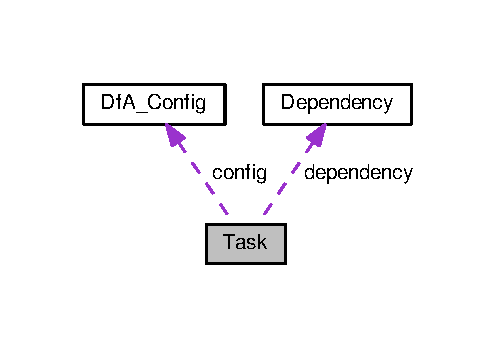
\includegraphics[width=239pt]{classTask__coll__graph}
\end{center}
\end{figure}
\subsection*{Public Member Functions}
\begin{DoxyCompactItemize}
\item 
\hyperlink{classTask_a27670d3d842b1c4ab38d2eacd5f5a920}{Task} (string \hyperlink{classTask_a7a3b3f194a78e928cd9a88420676cfa2}{dataflow\+\_\+tag}, string \hyperlink{classTask_a013314768d0b474bcc567f1cb98a1c01}{transformation\+\_\+tag}, int ID, int \hyperlink{classTask_aa5e5de369b641d4a6d66bd468d47b28b}{sub\+\_\+id}=0, string hostname=dfa\+\_\+hostname, int port=dfa\+\_\+port)
\item 
int \hyperlink{classTask_a8cb9bc9ccfc534b6cdd42edf15bad98e}{begin} ()
\item 
int \hyperlink{classTask_ad6acbe7ba8643e046513bf8d66e5f578}{end} ()
\item 
\hyperlink{classDataset}{Dataset} \& \hyperlink{classTask_a618a7fb22a6e06cf918def06da96f777}{add\+\_\+dataset} (string dataset\+\_\+tag)
\item 
\hyperlink{classDataset}{Dataset} \& \hyperlink{classTask_a052ec7c44c26ed666d327eb1b34451d8}{add\+\_\+dataset\+\_\+with\+\_\+element\+\_\+value} (string dataset\+\_\+tag, string value)
\item 
\hyperlink{classDataset}{Dataset} \& \hyperlink{classTask_ad0eeaa007ee192d7866a101c93730ab7}{add\+\_\+dataset\+\_\+with\+\_\+element\+\_\+values} (string dataset\+\_\+tag, vector$<$ string $>$ values)
\item 
void \hyperlink{classTask_a5171db4ee3e3065b21fd8085debc5e7e}{add\+\_\+dependent\+\_\+transformation} (string \hyperlink{classTask_a013314768d0b474bcc567f1cb98a1c01}{transformation\+\_\+tag}, int transformation\+\_\+id)
\item 
void \hyperlink{classTask_a839d94a0d3191d6f6ca7caf4a92c140b}{add\+\_\+dependent\+\_\+transformation} (string \hyperlink{classTask_a013314768d0b474bcc567f1cb98a1c01}{transformation\+\_\+tag}, vector$<$ int $>$ transformation\+\_\+ids)
\item 
void \hyperlink{classTask_a2307623af7ceb989b236a2c5dd0f715c}{add\+\_\+dependent\+\_\+transformations} (vector$<$ string $>$ transformation\+\_\+tags, int transformation\+\_\+id)
\item 
void \hyperlink{classTask_a381ed34fcd5d4e429fde0bb56ae5553a}{add\+\_\+dependent\+\_\+transformations} (vector$<$ string $>$ transformation\+\_\+tags, vector$<$ int $>$ transformation\+\_\+ids)
\item 
void \hyperlink{classTask_aba1111f932df1f306dc581b51350fcac}{set\+\_\+workspace} (string \hyperlink{classTask_a9827ffbb7019894dffd2c27350613634}{workspace})
\item 
void \hyperlink{classTask_a60c02d44aeaae258738b5e65e945736b}{set\+\_\+resource} (string \hyperlink{classTask_af5b241fe56a17e15d824ac7b57501f72}{resource})
\item 
void \hyperlink{classTask_ac89f5349a2b63b6362a30f2488b39ad9}{set\+\_\+status} (task\+\_\+status \hyperlink{classTask_ae814b4785e245eb50a6b5a745408a271}{status})
\item 
void \hyperlink{classTask_a943ea609e9e335120a40ed8b3d2adad8}{set\+\_\+sub\+\_\+id} (int \hyperlink{classTask_aa5e5de369b641d4a6d66bd468d47b28b}{sub\+\_\+id})
\item 
int \hyperlink{classTask_a40694bba7094fa408d1bd2f6ffb1c2ae}{get\+\_\+id} ()
\item 
int \hyperlink{classTask_ac614b1c136949a316a3a18253df0121d}{get\+\_\+sub\+\_\+id} ()
\item 
string \hyperlink{classTask_a7ec0e1dbe84fcb2fd338d29efe22012f}{get\+\_\+dataflow\+\_\+tag} ()
\item 
string \hyperlink{classTask_ac0821d83651e5702218f7cb414888915}{get\+\_\+transformation\+\_\+tag} ()
\item 
string \hyperlink{classTask_a19596eec4c5c3d12b4bba38a66bf21c2}{get\+\_\+workspace} ()
\item 
string \hyperlink{classTask_a1275490d93daa52ade635a9121e0a5dd}{get\+\_\+resource} ()
\item 
\hyperlink{classDataset}{Dataset} \& \hyperlink{classTask_af540b03cc9ed9910200895bbc080e911}{get\+\_\+dataset\+\_\+by\+\_\+tag} (string tag)
\item 
string \hyperlink{classTask_ae350debd8a8397e2923a164af6508010}{get\+\_\+status} ()
\item 
\hyperlink{classDependency}{Dependency} \& \hyperlink{classTask_ae69363e2ebfc402468ea97d29c89653a}{get\+\_\+dependency} ()
\item 
string \hyperlink{classTask_a80fb64595e226c3501313e85290fcaf2}{get\+\_\+specification} ()
\end{DoxyCompactItemize}
\subsection*{Protected Member Functions}
\begin{DoxyCompactItemize}
\item 
void \hyperlink{classTask_a404469dca46fda1c94e819345bd478e3}{add\+\_\+dependent\+\_\+transformation\+\_\+tag} (string \hyperlink{classTask_a013314768d0b474bcc567f1cb98a1c01}{transformation\+\_\+tag})
\item 
void \hyperlink{classTask_a861c0dc321a4b0e77f7cbe89dc7da75c}{add\+\_\+dependent\+\_\+transformation\+\_\+tags} (vector$<$ string $>$ transformation\+\_\+tags)
\item 
void \hyperlink{classTask_abe2b72a98501ca9554dd2aa18fad3245}{add\+\_\+dependent\+\_\+transformation\+\_\+id} (int task\+\_\+id)
\item 
void \hyperlink{classTask_ad549fad4fb70003b2f75bf3ae5a41d46}{add\+\_\+dependent\+\_\+transformation\+\_\+ids} (vector$<$ int $>$ task\+\_\+ids)
\item 
void \hyperlink{classTask_ad84f8f6e846b853c5e6b35ba3f0c470f}{insert\+\_\+dataset} (string dataset\+\_\+tag)
\item 
string \hyperlink{classTask_ae9ca005a8b6d0d3d794a7037f517ea20}{get\+\_\+post\+\_\+message} ()
\item 
void \hyperlink{classTask_a139cdf67c69c188c1a3ccc259d01da33}{save} ()
\end{DoxyCompactItemize}
\subsection*{Protected Attributes}
\begin{DoxyCompactItemize}
\item 
\mbox{\Hypertarget{classTask_a4b37b74b87a4419297e52180e715152c}\label{classTask_a4b37b74b87a4419297e52180e715152c}} 
\hyperlink{structDfA__Config}{Df\+A\+\_\+\+Config} \hyperlink{classTask_a4b37b74b87a4419297e52180e715152c}{config}
\begin{DoxyCompactList}\small\item\em Df\+Analyzer configurations. \end{DoxyCompactList}\item 
\mbox{\Hypertarget{classTask_a1bdc8139dd647f9701e9f43e588749d7}\label{classTask_a1bdc8139dd647f9701e9f43e588749d7}} 
int \hyperlink{classTask_a1bdc8139dd647f9701e9f43e588749d7}{id}
\begin{DoxyCompactList}\small\item\em task identifier \end{DoxyCompactList}\item 
\mbox{\Hypertarget{classTask_aa5e5de369b641d4a6d66bd468d47b28b}\label{classTask_aa5e5de369b641d4a6d66bd468d47b28b}} 
int \hyperlink{classTask_aa5e5de369b641d4a6d66bd468d47b28b}{sub\+\_\+id}
\begin{DoxyCompactList}\small\item\em task subidentifier \end{DoxyCompactList}\item 
\mbox{\Hypertarget{classTask_a7a3b3f194a78e928cd9a88420676cfa2}\label{classTask_a7a3b3f194a78e928cd9a88420676cfa2}} 
string \hyperlink{classTask_a7a3b3f194a78e928cd9a88420676cfa2}{dataflow\+\_\+tag}
\begin{DoxyCompactList}\small\item\em dataflow tag \end{DoxyCompactList}\item 
\mbox{\Hypertarget{classTask_a013314768d0b474bcc567f1cb98a1c01}\label{classTask_a013314768d0b474bcc567f1cb98a1c01}} 
string \hyperlink{classTask_a013314768d0b474bcc567f1cb98a1c01}{transformation\+\_\+tag}
\begin{DoxyCompactList}\small\item\em transformation tag \end{DoxyCompactList}\item 
\mbox{\Hypertarget{classTask_a9827ffbb7019894dffd2c27350613634}\label{classTask_a9827ffbb7019894dffd2c27350613634}} 
string \hyperlink{classTask_a9827ffbb7019894dffd2c27350613634}{workspace}
\begin{DoxyCompactList}\small\item\em workspace \end{DoxyCompactList}\item 
\mbox{\Hypertarget{classTask_a531bf480558a3ee2d9554fc0d91bafd3}\label{classTask_a531bf480558a3ee2d9554fc0d91bafd3}} 
map$<$ string, \hyperlink{classDataset}{Dataset} $>$ \hyperlink{classTask_a531bf480558a3ee2d9554fc0d91bafd3}{datasets}
\begin{DoxyCompactList}\small\item\em map of dataset tag with its object derived from \hyperlink{classDataset}{Dataset} \end{DoxyCompactList}\item 
\mbox{\Hypertarget{classTask_af5b241fe56a17e15d824ac7b57501f72}\label{classTask_af5b241fe56a17e15d824ac7b57501f72}} 
string \hyperlink{classTask_af5b241fe56a17e15d824ac7b57501f72}{resource}
\begin{DoxyCompactList}\small\item\em resource \end{DoxyCompactList}\item 
\mbox{\Hypertarget{classTask_ae814b4785e245eb50a6b5a745408a271}\label{classTask_ae814b4785e245eb50a6b5a745408a271}} 
task\+\_\+status \hyperlink{classTask_ae814b4785e245eb50a6b5a745408a271}{status}
\begin{DoxyCompactList}\small\item\em task status, which can be R\+E\+A\+DY, R\+U\+N\+N\+I\+NG, or F\+I\+N\+I\+S\+H\+ED \end{DoxyCompactList}\item 
\mbox{\Hypertarget{classTask_a3646beab5c494e230601630dc5ffe27d}\label{classTask_a3646beab5c494e230601630dc5ffe27d}} 
\hyperlink{classDependency}{Dependency} \hyperlink{classTask_a3646beab5c494e230601630dc5ffe27d}{dependency}
\begin{DoxyCompactList}\small\item\em data dependency \end{DoxyCompactList}\end{DoxyCompactItemize}


\subsection{Detailed Description}
Class to represent a task (retrospective provenance). 

\subsection{Constructor \& Destructor Documentation}
\mbox{\Hypertarget{classTask_a27670d3d842b1c4ab38d2eacd5f5a920}\label{classTask_a27670d3d842b1c4ab38d2eacd5f5a920}} 
\index{Task@{Task}!Task@{Task}}
\index{Task@{Task}!Task@{Task}}
\subsubsection{\texorpdfstring{Task()}{Task()}}
{\footnotesize\ttfamily Task\+::\+Task (\begin{DoxyParamCaption}\item[{string}]{dataflow\+\_\+tag,  }\item[{string}]{transformation\+\_\+tag,  }\item[{int}]{ID,  }\item[{int}]{sub\+\_\+id = {\ttfamily 0},  }\item[{string}]{hostname = {\ttfamily dfa\+\_\+hostname},  }\item[{int}]{port = {\ttfamily dfa\+\_\+port} }\end{DoxyParamCaption})\hspace{0.3cm}{\ttfamily [inline]}}

Constructor of a task. 
\begin{DoxyParams}{Parameters}
{\em dataflow\+\_\+tag} & a dataflow tag \\
\hline
{\em transformation\+\_\+tag} & a transformation tag \\
\hline
{\em ID} & a task identifier \\
\hline
{\em sub\+\_\+id} & a task subidentifier (optional) \\
\hline
{\em hostname} & a hostname to the Df\+Analyzer server (optional) \\
\hline
{\em port} & a port to the Df\+Analyzer server (optional) \\
\hline
\end{DoxyParams}


\subsection{Member Function Documentation}
\mbox{\Hypertarget{classTask_a618a7fb22a6e06cf918def06da96f777}\label{classTask_a618a7fb22a6e06cf918def06da96f777}} 
\index{Task@{Task}!add\+\_\+dataset@{add\+\_\+dataset}}
\index{add\+\_\+dataset@{add\+\_\+dataset}!Task@{Task}}
\subsubsection{\texorpdfstring{add\+\_\+dataset()}{add\_dataset()}}
{\footnotesize\ttfamily \hyperlink{classDataset}{Dataset} \& Task\+::add\+\_\+dataset (\begin{DoxyParamCaption}\item[{string}]{dataset\+\_\+tag }\end{DoxyParamCaption})}

Add a dataset to the task. 
\begin{DoxyParams}{Parameters}
{\em dataset\+\_\+tag} & a dataset tag \\
\hline
\end{DoxyParams}
\mbox{\Hypertarget{classTask_a052ec7c44c26ed666d327eb1b34451d8}\label{classTask_a052ec7c44c26ed666d327eb1b34451d8}} 
\index{Task@{Task}!add\+\_\+dataset\+\_\+with\+\_\+element\+\_\+value@{add\+\_\+dataset\+\_\+with\+\_\+element\+\_\+value}}
\index{add\+\_\+dataset\+\_\+with\+\_\+element\+\_\+value@{add\+\_\+dataset\+\_\+with\+\_\+element\+\_\+value}!Task@{Task}}
\subsubsection{\texorpdfstring{add\+\_\+dataset\+\_\+with\+\_\+element\+\_\+value()}{add\_dataset\_with\_element\_value()}}
{\footnotesize\ttfamily \hyperlink{classDataset}{Dataset} \& Task\+::add\+\_\+dataset\+\_\+with\+\_\+element\+\_\+value (\begin{DoxyParamCaption}\item[{string}]{dataset\+\_\+tag,  }\item[{string}]{value }\end{DoxyParamCaption})}

Add a dataset to the task with a single attribute value. 
\begin{DoxyParams}{Parameters}
{\em dataset\+\_\+tag} & a dataset tag \\
\hline
{\em value} & a single attribute value \\
\hline
\end{DoxyParams}
\mbox{\Hypertarget{classTask_ad0eeaa007ee192d7866a101c93730ab7}\label{classTask_ad0eeaa007ee192d7866a101c93730ab7}} 
\index{Task@{Task}!add\+\_\+dataset\+\_\+with\+\_\+element\+\_\+values@{add\+\_\+dataset\+\_\+with\+\_\+element\+\_\+values}}
\index{add\+\_\+dataset\+\_\+with\+\_\+element\+\_\+values@{add\+\_\+dataset\+\_\+with\+\_\+element\+\_\+values}!Task@{Task}}
\subsubsection{\texorpdfstring{add\+\_\+dataset\+\_\+with\+\_\+element\+\_\+values()}{add\_dataset\_with\_element\_values()}}
{\footnotesize\ttfamily \hyperlink{classDataset}{Dataset} \& Task\+::add\+\_\+dataset\+\_\+with\+\_\+element\+\_\+values (\begin{DoxyParamCaption}\item[{string}]{dataset\+\_\+tag,  }\item[{vector$<$ string $>$}]{values }\end{DoxyParamCaption})}

Add a dataset to the task with multiple attribute values. 
\begin{DoxyParams}{Parameters}
{\em dataset\+\_\+tag} & a dataset tag \\
\hline
{\em values} & a set of attribute values \\
\hline
\end{DoxyParams}
\mbox{\Hypertarget{classTask_a5171db4ee3e3065b21fd8085debc5e7e}\label{classTask_a5171db4ee3e3065b21fd8085debc5e7e}} 
\index{Task@{Task}!add\+\_\+dependent\+\_\+transformation@{add\+\_\+dependent\+\_\+transformation}}
\index{add\+\_\+dependent\+\_\+transformation@{add\+\_\+dependent\+\_\+transformation}!Task@{Task}}
\subsubsection{\texorpdfstring{add\+\_\+dependent\+\_\+transformation()}{add\_dependent\_transformation()}\hspace{0.1cm}{\footnotesize\ttfamily [1/2]}}
{\footnotesize\ttfamily void Task\+::add\+\_\+dependent\+\_\+transformation (\begin{DoxyParamCaption}\item[{string}]{transformation\+\_\+tag,  }\item[{int}]{transformation\+\_\+id }\end{DoxyParamCaption})}

Add a dependent transformation to the task with a single dependent task. 
\begin{DoxyParams}{Parameters}
{\em transformation\+\_\+tag} & a transformation tag \\
\hline
{\em transformation\+\_\+id} & a transformation identifier \\
\hline
\end{DoxyParams}
\mbox{\Hypertarget{classTask_a839d94a0d3191d6f6ca7caf4a92c140b}\label{classTask_a839d94a0d3191d6f6ca7caf4a92c140b}} 
\index{Task@{Task}!add\+\_\+dependent\+\_\+transformation@{add\+\_\+dependent\+\_\+transformation}}
\index{add\+\_\+dependent\+\_\+transformation@{add\+\_\+dependent\+\_\+transformation}!Task@{Task}}
\subsubsection{\texorpdfstring{add\+\_\+dependent\+\_\+transformation()}{add\_dependent\_transformation()}\hspace{0.1cm}{\footnotesize\ttfamily [2/2]}}
{\footnotesize\ttfamily void Task\+::add\+\_\+dependent\+\_\+transformation (\begin{DoxyParamCaption}\item[{string}]{transformation\+\_\+tag,  }\item[{vector$<$ int $>$}]{transformation\+\_\+ids }\end{DoxyParamCaption})}

Add a dependent transformation to the task with multiple dependent tasks. 
\begin{DoxyParams}{Parameters}
{\em transformation\+\_\+tag} & a transformation tag \\
\hline
{\em transformation\+\_\+ids} & a set of transformation identifiers \\
\hline
\end{DoxyParams}
\mbox{\Hypertarget{classTask_abe2b72a98501ca9554dd2aa18fad3245}\label{classTask_abe2b72a98501ca9554dd2aa18fad3245}} 
\index{Task@{Task}!add\+\_\+dependent\+\_\+transformation\+\_\+id@{add\+\_\+dependent\+\_\+transformation\+\_\+id}}
\index{add\+\_\+dependent\+\_\+transformation\+\_\+id@{add\+\_\+dependent\+\_\+transformation\+\_\+id}!Task@{Task}}
\subsubsection{\texorpdfstring{add\+\_\+dependent\+\_\+transformation\+\_\+id()}{add\_dependent\_transformation\_id()}}
{\footnotesize\ttfamily void Task\+::add\+\_\+dependent\+\_\+transformation\+\_\+id (\begin{DoxyParamCaption}\item[{int}]{task\+\_\+id }\end{DoxyParamCaption})\hspace{0.3cm}{\ttfamily [protected]}}

Add a dependent task identifier to the dependent transformation tag. 
\begin{DoxyParams}{Parameters}
{\em task\+\_\+id} & a task identifier \\
\hline
\end{DoxyParams}
\mbox{\Hypertarget{classTask_ad549fad4fb70003b2f75bf3ae5a41d46}\label{classTask_ad549fad4fb70003b2f75bf3ae5a41d46}} 
\index{Task@{Task}!add\+\_\+dependent\+\_\+transformation\+\_\+ids@{add\+\_\+dependent\+\_\+transformation\+\_\+ids}}
\index{add\+\_\+dependent\+\_\+transformation\+\_\+ids@{add\+\_\+dependent\+\_\+transformation\+\_\+ids}!Task@{Task}}
\subsubsection{\texorpdfstring{add\+\_\+dependent\+\_\+transformation\+\_\+ids()}{add\_dependent\_transformation\_ids()}}
{\footnotesize\ttfamily void Task\+::add\+\_\+dependent\+\_\+transformation\+\_\+ids (\begin{DoxyParamCaption}\item[{vector$<$ int $>$}]{task\+\_\+ids }\end{DoxyParamCaption})\hspace{0.3cm}{\ttfamily [protected]}}

Add a set of dependent task identifiers to the dependent transformation tags. 
\begin{DoxyParams}{Parameters}
{\em task\+\_\+ids} & a set of task identifiers \\
\hline
\end{DoxyParams}
\mbox{\Hypertarget{classTask_a404469dca46fda1c94e819345bd478e3}\label{classTask_a404469dca46fda1c94e819345bd478e3}} 
\index{Task@{Task}!add\+\_\+dependent\+\_\+transformation\+\_\+tag@{add\+\_\+dependent\+\_\+transformation\+\_\+tag}}
\index{add\+\_\+dependent\+\_\+transformation\+\_\+tag@{add\+\_\+dependent\+\_\+transformation\+\_\+tag}!Task@{Task}}
\subsubsection{\texorpdfstring{add\+\_\+dependent\+\_\+transformation\+\_\+tag()}{add\_dependent\_transformation\_tag()}}
{\footnotesize\ttfamily void Task\+::add\+\_\+dependent\+\_\+transformation\+\_\+tag (\begin{DoxyParamCaption}\item[{string}]{transformation\+\_\+tag }\end{DoxyParamCaption})\hspace{0.3cm}{\ttfamily [protected]}}

Add a dependent transformation tag. 
\begin{DoxyParams}{Parameters}
{\em transformation\+\_\+tag} & a transformation tag \\
\hline
\end{DoxyParams}
\mbox{\Hypertarget{classTask_a861c0dc321a4b0e77f7cbe89dc7da75c}\label{classTask_a861c0dc321a4b0e77f7cbe89dc7da75c}} 
\index{Task@{Task}!add\+\_\+dependent\+\_\+transformation\+\_\+tags@{add\+\_\+dependent\+\_\+transformation\+\_\+tags}}
\index{add\+\_\+dependent\+\_\+transformation\+\_\+tags@{add\+\_\+dependent\+\_\+transformation\+\_\+tags}!Task@{Task}}
\subsubsection{\texorpdfstring{add\+\_\+dependent\+\_\+transformation\+\_\+tags()}{add\_dependent\_transformation\_tags()}}
{\footnotesize\ttfamily void Task\+::add\+\_\+dependent\+\_\+transformation\+\_\+tags (\begin{DoxyParamCaption}\item[{vector$<$ string $>$}]{transformation\+\_\+tags }\end{DoxyParamCaption})\hspace{0.3cm}{\ttfamily [protected]}}

Add a set of dependent transformation tags. 
\begin{DoxyParams}{Parameters}
{\em transformation\+\_\+tags} & a set of dependent transformation tags \\
\hline
\end{DoxyParams}
\mbox{\Hypertarget{classTask_a2307623af7ceb989b236a2c5dd0f715c}\label{classTask_a2307623af7ceb989b236a2c5dd0f715c}} 
\index{Task@{Task}!add\+\_\+dependent\+\_\+transformations@{add\+\_\+dependent\+\_\+transformations}}
\index{add\+\_\+dependent\+\_\+transformations@{add\+\_\+dependent\+\_\+transformations}!Task@{Task}}
\subsubsection{\texorpdfstring{add\+\_\+dependent\+\_\+transformations()}{add\_dependent\_transformations()}\hspace{0.1cm}{\footnotesize\ttfamily [1/2]}}
{\footnotesize\ttfamily void Task\+::add\+\_\+dependent\+\_\+transformations (\begin{DoxyParamCaption}\item[{vector$<$ string $>$}]{transformation\+\_\+tags,  }\item[{int}]{transformation\+\_\+id }\end{DoxyParamCaption})}

Add a set of dependent transformations to the task with a single dependent task. 
\begin{DoxyParams}{Parameters}
{\em transformation\+\_\+tags} & a set of transformation tags \\
\hline
{\em transformation\+\_\+id} & a transformation identifier \\
\hline
\end{DoxyParams}
\mbox{\Hypertarget{classTask_a381ed34fcd5d4e429fde0bb56ae5553a}\label{classTask_a381ed34fcd5d4e429fde0bb56ae5553a}} 
\index{Task@{Task}!add\+\_\+dependent\+\_\+transformations@{add\+\_\+dependent\+\_\+transformations}}
\index{add\+\_\+dependent\+\_\+transformations@{add\+\_\+dependent\+\_\+transformations}!Task@{Task}}
\subsubsection{\texorpdfstring{add\+\_\+dependent\+\_\+transformations()}{add\_dependent\_transformations()}\hspace{0.1cm}{\footnotesize\ttfamily [2/2]}}
{\footnotesize\ttfamily void Task\+::add\+\_\+dependent\+\_\+transformations (\begin{DoxyParamCaption}\item[{vector$<$ string $>$}]{transformation\+\_\+tags,  }\item[{vector$<$ int $>$}]{transformation\+\_\+ids }\end{DoxyParamCaption})}

Add a set of dependent transformations to the task with multiple dependent tasks. 
\begin{DoxyParams}{Parameters}
{\em transformation\+\_\+tags} & a set of transformation tags \\
\hline
{\em transformation\+\_\+ids} & a set of transformation identifiers \\
\hline
\end{DoxyParams}
\mbox{\Hypertarget{classTask_a8cb9bc9ccfc534b6cdd42edf15bad98e}\label{classTask_a8cb9bc9ccfc534b6cdd42edf15bad98e}} 
\index{Task@{Task}!begin@{begin}}
\index{begin@{begin}!Task@{Task}}
\subsubsection{\texorpdfstring{begin()}{begin()}}
{\footnotesize\ttfamily int Task\+::begin (\begin{DoxyParamCaption}{ }\end{DoxyParamCaption})}

Save a task with the status R\+U\+N\+N\+I\+NG. \begin{DoxyReturn}{Returns}
the exit status code of the H\+T\+TP request sent using curl. 
\end{DoxyReturn}
\mbox{\Hypertarget{classTask_ad6acbe7ba8643e046513bf8d66e5f578}\label{classTask_ad6acbe7ba8643e046513bf8d66e5f578}} 
\index{Task@{Task}!end@{end}}
\index{end@{end}!Task@{Task}}
\subsubsection{\texorpdfstring{end()}{end()}}
{\footnotesize\ttfamily int Task\+::end (\begin{DoxyParamCaption}{ }\end{DoxyParamCaption})}

Save a task with the status F\+I\+N\+I\+S\+H\+ED. \begin{DoxyReturn}{Returns}
the exit status code of the H\+T\+TP request sent using curl. 
\end{DoxyReturn}
\mbox{\Hypertarget{classTask_a7ec0e1dbe84fcb2fd338d29efe22012f}\label{classTask_a7ec0e1dbe84fcb2fd338d29efe22012f}} 
\index{Task@{Task}!get\+\_\+dataflow\+\_\+tag@{get\+\_\+dataflow\+\_\+tag}}
\index{get\+\_\+dataflow\+\_\+tag@{get\+\_\+dataflow\+\_\+tag}!Task@{Task}}
\subsubsection{\texorpdfstring{get\+\_\+dataflow\+\_\+tag()}{get\_dataflow\_tag()}}
{\footnotesize\ttfamily string Task\+::get\+\_\+dataflow\+\_\+tag (\begin{DoxyParamCaption}{ }\end{DoxyParamCaption})}

Get dataflow tag. \begin{DoxyReturn}{Returns}
the dataflow tag 
\end{DoxyReturn}
\mbox{\Hypertarget{classTask_af540b03cc9ed9910200895bbc080e911}\label{classTask_af540b03cc9ed9910200895bbc080e911}} 
\index{Task@{Task}!get\+\_\+dataset\+\_\+by\+\_\+tag@{get\+\_\+dataset\+\_\+by\+\_\+tag}}
\index{get\+\_\+dataset\+\_\+by\+\_\+tag@{get\+\_\+dataset\+\_\+by\+\_\+tag}!Task@{Task}}
\subsubsection{\texorpdfstring{get\+\_\+dataset\+\_\+by\+\_\+tag()}{get\_dataset\_by\_tag()}}
{\footnotesize\ttfamily \hyperlink{classDataset}{Dataset} \& Task\+::get\+\_\+dataset\+\_\+by\+\_\+tag (\begin{DoxyParamCaption}\item[{string}]{tag }\end{DoxyParamCaption})}

Get dataset given a tag. 
\begin{DoxyParams}{Parameters}
{\em tag} & a dataset tag. \\
\hline
\end{DoxyParams}
\begin{DoxyReturn}{Returns}
the reference of the dataset given a tag 
\end{DoxyReturn}
\mbox{\Hypertarget{classTask_ae69363e2ebfc402468ea97d29c89653a}\label{classTask_ae69363e2ebfc402468ea97d29c89653a}} 
\index{Task@{Task}!get\+\_\+dependency@{get\+\_\+dependency}}
\index{get\+\_\+dependency@{get\+\_\+dependency}!Task@{Task}}
\subsubsection{\texorpdfstring{get\+\_\+dependency()}{get\_dependency()}}
{\footnotesize\ttfamily \hyperlink{classDependency}{Dependency} \& Task\+::get\+\_\+dependency (\begin{DoxyParamCaption}{ }\end{DoxyParamCaption})}

Get the data dependency. \begin{DoxyReturn}{Returns}
the data dependency 
\end{DoxyReturn}
\mbox{\Hypertarget{classTask_a40694bba7094fa408d1bd2f6ffb1c2ae}\label{classTask_a40694bba7094fa408d1bd2f6ffb1c2ae}} 
\index{Task@{Task}!get\+\_\+id@{get\+\_\+id}}
\index{get\+\_\+id@{get\+\_\+id}!Task@{Task}}
\subsubsection{\texorpdfstring{get\+\_\+id()}{get\_id()}}
{\footnotesize\ttfamily int Task\+::get\+\_\+id (\begin{DoxyParamCaption}{ }\end{DoxyParamCaption})}

Get task identifier. \begin{DoxyReturn}{Returns}
the task identifier 
\end{DoxyReturn}
\mbox{\Hypertarget{classTask_ae9ca005a8b6d0d3d794a7037f517ea20}\label{classTask_ae9ca005a8b6d0d3d794a7037f517ea20}} 
\index{Task@{Task}!get\+\_\+post\+\_\+message@{get\+\_\+post\+\_\+message}}
\index{get\+\_\+post\+\_\+message@{get\+\_\+post\+\_\+message}!Task@{Task}}
\subsubsection{\texorpdfstring{get\+\_\+post\+\_\+message()}{get\_post\_message()}}
{\footnotesize\ttfamily string Task\+::get\+\_\+post\+\_\+message (\begin{DoxyParamCaption}{ }\end{DoxyParamCaption})\hspace{0.3cm}{\ttfamily [protected]}}

Get message to be sent to Df\+Analyzer server using an H\+T\+TP request with P\+O\+ST method. \begin{DoxyReturn}{Returns}
the message in H\+T\+TP request 
\end{DoxyReturn}
\mbox{\Hypertarget{classTask_a1275490d93daa52ade635a9121e0a5dd}\label{classTask_a1275490d93daa52ade635a9121e0a5dd}} 
\index{Task@{Task}!get\+\_\+resource@{get\+\_\+resource}}
\index{get\+\_\+resource@{get\+\_\+resource}!Task@{Task}}
\subsubsection{\texorpdfstring{get\+\_\+resource()}{get\_resource()}}
{\footnotesize\ttfamily string Task\+::get\+\_\+resource (\begin{DoxyParamCaption}{ }\end{DoxyParamCaption})}

Get the resource \begin{DoxyReturn}{Returns}
the resource 
\end{DoxyReturn}
\mbox{\Hypertarget{classTask_a80fb64595e226c3501313e85290fcaf2}\label{classTask_a80fb64595e226c3501313e85290fcaf2}} 
\index{Task@{Task}!get\+\_\+specification@{get\+\_\+specification}}
\index{get\+\_\+specification@{get\+\_\+specification}!Task@{Task}}
\subsubsection{\texorpdfstring{get\+\_\+specification()}{get\_specification()}}
{\footnotesize\ttfamily string Task\+::get\+\_\+specification (\begin{DoxyParamCaption}{ }\end{DoxyParamCaption})}

Get task specification. \begin{DoxyReturn}{Returns}
the task specification as a string 
\end{DoxyReturn}
\mbox{\Hypertarget{classTask_ae350debd8a8397e2923a164af6508010}\label{classTask_ae350debd8a8397e2923a164af6508010}} 
\index{Task@{Task}!get\+\_\+status@{get\+\_\+status}}
\index{get\+\_\+status@{get\+\_\+status}!Task@{Task}}
\subsubsection{\texorpdfstring{get\+\_\+status()}{get\_status()}}
{\footnotesize\ttfamily string Task\+::get\+\_\+status (\begin{DoxyParamCaption}{ }\end{DoxyParamCaption})}

Get the task status. \begin{DoxyReturn}{Returns}
the task status 
\end{DoxyReturn}
\mbox{\Hypertarget{classTask_ac614b1c136949a316a3a18253df0121d}\label{classTask_ac614b1c136949a316a3a18253df0121d}} 
\index{Task@{Task}!get\+\_\+sub\+\_\+id@{get\+\_\+sub\+\_\+id}}
\index{get\+\_\+sub\+\_\+id@{get\+\_\+sub\+\_\+id}!Task@{Task}}
\subsubsection{\texorpdfstring{get\+\_\+sub\+\_\+id()}{get\_sub\_id()}}
{\footnotesize\ttfamily int Task\+::get\+\_\+sub\+\_\+id (\begin{DoxyParamCaption}{ }\end{DoxyParamCaption})}

Get task subidentifier. \begin{DoxyReturn}{Returns}
the task subidentifier 
\end{DoxyReturn}
\mbox{\Hypertarget{classTask_ac0821d83651e5702218f7cb414888915}\label{classTask_ac0821d83651e5702218f7cb414888915}} 
\index{Task@{Task}!get\+\_\+transformation\+\_\+tag@{get\+\_\+transformation\+\_\+tag}}
\index{get\+\_\+transformation\+\_\+tag@{get\+\_\+transformation\+\_\+tag}!Task@{Task}}
\subsubsection{\texorpdfstring{get\+\_\+transformation\+\_\+tag()}{get\_transformation\_tag()}}
{\footnotesize\ttfamily string Task\+::get\+\_\+transformation\+\_\+tag (\begin{DoxyParamCaption}{ }\end{DoxyParamCaption})}

Get transformation tag. \begin{DoxyReturn}{Returns}
the transformation tag 
\end{DoxyReturn}
\mbox{\Hypertarget{classTask_a19596eec4c5c3d12b4bba38a66bf21c2}\label{classTask_a19596eec4c5c3d12b4bba38a66bf21c2}} 
\index{Task@{Task}!get\+\_\+workspace@{get\+\_\+workspace}}
\index{get\+\_\+workspace@{get\+\_\+workspace}!Task@{Task}}
\subsubsection{\texorpdfstring{get\+\_\+workspace()}{get\_workspace()}}
{\footnotesize\ttfamily string Task\+::get\+\_\+workspace (\begin{DoxyParamCaption}{ }\end{DoxyParamCaption})}

Get the workspace. \begin{DoxyReturn}{Returns}
the workspace 
\end{DoxyReturn}
\mbox{\Hypertarget{classTask_ad84f8f6e846b853c5e6b35ba3f0c470f}\label{classTask_ad84f8f6e846b853c5e6b35ba3f0c470f}} 
\index{Task@{Task}!insert\+\_\+dataset@{insert\+\_\+dataset}}
\index{insert\+\_\+dataset@{insert\+\_\+dataset}!Task@{Task}}
\subsubsection{\texorpdfstring{insert\+\_\+dataset()}{insert\_dataset()}}
{\footnotesize\ttfamily void Task\+::insert\+\_\+dataset (\begin{DoxyParamCaption}\item[{string}]{dataset\+\_\+tag }\end{DoxyParamCaption})\hspace{0.3cm}{\ttfamily [protected]}}

Insert dataset consumed/produced by the task. 
\begin{DoxyParams}{Parameters}
{\em dataset\+\_\+tag} & a dataset tag \\
\hline
\end{DoxyParams}
\mbox{\Hypertarget{classTask_a139cdf67c69c188c1a3ccc259d01da33}\label{classTask_a139cdf67c69c188c1a3ccc259d01da33}} 
\index{Task@{Task}!save@{save}}
\index{save@{save}!Task@{Task}}
\subsubsection{\texorpdfstring{save()}{save()}}
{\footnotesize\ttfamily void Task\+::save (\begin{DoxyParamCaption}{ }\end{DoxyParamCaption})\hspace{0.3cm}{\ttfamily [protected]}}

Save a task in Df\+Analyzer database. \mbox{\Hypertarget{classTask_a60c02d44aeaae258738b5e65e945736b}\label{classTask_a60c02d44aeaae258738b5e65e945736b}} 
\index{Task@{Task}!set\+\_\+resource@{set\+\_\+resource}}
\index{set\+\_\+resource@{set\+\_\+resource}!Task@{Task}}
\subsubsection{\texorpdfstring{set\+\_\+resource()}{set\_resource()}}
{\footnotesize\ttfamily void Task\+::set\+\_\+resource (\begin{DoxyParamCaption}\item[{string}]{resource }\end{DoxyParamCaption})}

\hyperlink{classSet}{Set} resource. 
\begin{DoxyParams}{Parameters}
{\em resource} & a resource \\
\hline
\end{DoxyParams}
\mbox{\Hypertarget{classTask_ac89f5349a2b63b6362a30f2488b39ad9}\label{classTask_ac89f5349a2b63b6362a30f2488b39ad9}} 
\index{Task@{Task}!set\+\_\+status@{set\+\_\+status}}
\index{set\+\_\+status@{set\+\_\+status}!Task@{Task}}
\subsubsection{\texorpdfstring{set\+\_\+status()}{set\_status()}}
{\footnotesize\ttfamily void Task\+::set\+\_\+status (\begin{DoxyParamCaption}\item[{task\+\_\+status}]{status }\end{DoxyParamCaption})}

\hyperlink{classSet}{Set} task status. 
\begin{DoxyParams}{Parameters}
{\em status} & a task status \\
\hline
\end{DoxyParams}
\mbox{\Hypertarget{classTask_a943ea609e9e335120a40ed8b3d2adad8}\label{classTask_a943ea609e9e335120a40ed8b3d2adad8}} 
\index{Task@{Task}!set\+\_\+sub\+\_\+id@{set\+\_\+sub\+\_\+id}}
\index{set\+\_\+sub\+\_\+id@{set\+\_\+sub\+\_\+id}!Task@{Task}}
\subsubsection{\texorpdfstring{set\+\_\+sub\+\_\+id()}{set\_sub\_id()}}
{\footnotesize\ttfamily void Task\+::set\+\_\+sub\+\_\+id (\begin{DoxyParamCaption}\item[{int}]{sub\+\_\+id }\end{DoxyParamCaption})}

\hyperlink{classSet}{Set} task subidentifier. 
\begin{DoxyParams}{Parameters}
{\em sub\+\_\+id} & a task subidentifier \\
\hline
\end{DoxyParams}
\mbox{\Hypertarget{classTask_aba1111f932df1f306dc581b51350fcac}\label{classTask_aba1111f932df1f306dc581b51350fcac}} 
\index{Task@{Task}!set\+\_\+workspace@{set\+\_\+workspace}}
\index{set\+\_\+workspace@{set\+\_\+workspace}!Task@{Task}}
\subsubsection{\texorpdfstring{set\+\_\+workspace()}{set\_workspace()}}
{\footnotesize\ttfamily void Task\+::set\+\_\+workspace (\begin{DoxyParamCaption}\item[{string}]{workspace }\end{DoxyParamCaption})}

\hyperlink{classSet}{Set} workspace. 
\begin{DoxyParams}{Parameters}
{\em workspace} & a workspace \\
\hline
\end{DoxyParams}


The documentation for this class was generated from the following files\+:\begin{DoxyCompactItemize}
\item 
include/task.\+h\item 
src/task.\+cpp\end{DoxyCompactItemize}

\hypertarget{classTransformation}{}\section{Transformation Class Reference}
\label{classTransformation}\index{Transformation@{Transformation}}


{\ttfamily \#include $<$transformation.\+h$>$}

\subsection*{Public Member Functions}
\begin{DoxyCompactItemize}
\item 
\hyperlink{classTransformation_a7d309ec7b7e612c941982b0b3a484f70}{Transformation} (string \hyperlink{classTransformation_aae5fa5db90050f8bd2f24cce6864fb14}{tag})
\item 
void \hyperlink{classTransformation_a2a2af5b05352dd3d401c7af6027248d0}{add\+\_\+input\+\_\+set} (\hyperlink{classSet}{Set} set)
\item 
void \hyperlink{classTransformation_a63b5bc7696a22e413d95540703738894}{add\+\_\+output\+\_\+set} (\hyperlink{classSet}{Set} set)
\item 
string \hyperlink{classTransformation_a5ad25a244c9506d5bb89cfed8a3667b0}{get\+\_\+tag} ()
\item 
string \hyperlink{classTransformation_adfe87345cdc0ebff5a6212dd9779ec87}{get\+\_\+specification} ()
\item 
vector$<$ string $>$ \hyperlink{classTransformation_a96a5923535ff3663c478fdc0cd7ddc34}{get\+\_\+input\+\_\+sets} ()
\item 
vector$<$ string $>$ \hyperlink{classTransformation_a309852a4fbb5db261a1a6d564c7147c8}{get\+\_\+output\+\_\+sets} ()
\item 
void \hyperlink{classTransformation_a015a16690d152a99ddf482cb56c05e07}{set\+\_\+input\+\_\+sets} (vector$<$ \hyperlink{classSet}{Set} $>$ \hyperlink{classTransformation_a5cff8880aed2eaf0ad3bdc9ad1c86148}{input\+\_\+sets})
\item 
void \hyperlink{classTransformation_a10b3128bcb16deae76746a3179e8e315}{set\+\_\+output\+\_\+sets} (vector$<$ \hyperlink{classSet}{Set} $>$ \hyperlink{classTransformation_ac1a61ff0d71f8ceb2d4338d2abd04f24}{output\+\_\+sets})
\item 
bool \hyperlink{classTransformation_a86424a75814c92796a3dbd5530df7598}{has\+\_\+output\+\_\+set} (vector$<$ string $>$ dataset\+\_\+tags)
\end{DoxyCompactItemize}
\subsection*{Protected Attributes}
\begin{DoxyCompactItemize}
\item 
\mbox{\Hypertarget{classTransformation_aae5fa5db90050f8bd2f24cce6864fb14}\label{classTransformation_aae5fa5db90050f8bd2f24cce6864fb14}} 
string \hyperlink{classTransformation_aae5fa5db90050f8bd2f24cce6864fb14}{tag}
\begin{DoxyCompactList}\small\item\em data transformation tag \end{DoxyCompactList}\item 
\mbox{\Hypertarget{classTransformation_a5cff8880aed2eaf0ad3bdc9ad1c86148}\label{classTransformation_a5cff8880aed2eaf0ad3bdc9ad1c86148}} 
vector$<$ \hyperlink{classSet}{Set} $>$ \hyperlink{classTransformation_a5cff8880aed2eaf0ad3bdc9ad1c86148}{input\+\_\+sets}
\begin{DoxyCompactList}\small\item\em input datasets \end{DoxyCompactList}\item 
\mbox{\Hypertarget{classTransformation_ac1a61ff0d71f8ceb2d4338d2abd04f24}\label{classTransformation_ac1a61ff0d71f8ceb2d4338d2abd04f24}} 
vector$<$ \hyperlink{classSet}{Set} $>$ \hyperlink{classTransformation_ac1a61ff0d71f8ceb2d4338d2abd04f24}{output\+\_\+sets}
\begin{DoxyCompactList}\small\item\em output datasets \end{DoxyCompactList}\end{DoxyCompactItemize}


\subsection{Detailed Description}
Class to represent a data transformation specification (prospective provenance). 

\subsection{Constructor \& Destructor Documentation}
\mbox{\Hypertarget{classTransformation_a7d309ec7b7e612c941982b0b3a484f70}\label{classTransformation_a7d309ec7b7e612c941982b0b3a484f70}} 
\index{Transformation@{Transformation}!Transformation@{Transformation}}
\index{Transformation@{Transformation}!Transformation@{Transformation}}
\subsubsection{\texorpdfstring{Transformation()}{Transformation()}}
{\footnotesize\ttfamily Transformation\+::\+Transformation (\begin{DoxyParamCaption}\item[{string}]{tag }\end{DoxyParamCaption})\hspace{0.3cm}{\ttfamily [inline]}}

Constructor of a data transformation specification. 
\begin{DoxyParams}{Parameters}
{\em tag} & a data transformation specification. \\
\hline
\end{DoxyParams}


\subsection{Member Function Documentation}
\mbox{\Hypertarget{classTransformation_a2a2af5b05352dd3d401c7af6027248d0}\label{classTransformation_a2a2af5b05352dd3d401c7af6027248d0}} 
\index{Transformation@{Transformation}!add\+\_\+input\+\_\+set@{add\+\_\+input\+\_\+set}}
\index{add\+\_\+input\+\_\+set@{add\+\_\+input\+\_\+set}!Transformation@{Transformation}}
\subsubsection{\texorpdfstring{add\+\_\+input\+\_\+set()}{add\_input\_set()}}
{\footnotesize\ttfamily void Transformation\+::add\+\_\+input\+\_\+set (\begin{DoxyParamCaption}\item[{\hyperlink{classSet}{Set}}]{set }\end{DoxyParamCaption})}

Add an input dataset to data transformation specification. 
\begin{DoxyParams}{Parameters}
{\em set} & an input dataset specification. \\
\hline
\end{DoxyParams}
\mbox{\Hypertarget{classTransformation_a63b5bc7696a22e413d95540703738894}\label{classTransformation_a63b5bc7696a22e413d95540703738894}} 
\index{Transformation@{Transformation}!add\+\_\+output\+\_\+set@{add\+\_\+output\+\_\+set}}
\index{add\+\_\+output\+\_\+set@{add\+\_\+output\+\_\+set}!Transformation@{Transformation}}
\subsubsection{\texorpdfstring{add\+\_\+output\+\_\+set()}{add\_output\_set()}}
{\footnotesize\ttfamily void Transformation\+::add\+\_\+output\+\_\+set (\begin{DoxyParamCaption}\item[{\hyperlink{classSet}{Set}}]{set }\end{DoxyParamCaption})}

Add an output dataset to data transformation specification. 
\begin{DoxyParams}{Parameters}
{\em set} & an output dataset specification. \\
\hline
\end{DoxyParams}
\mbox{\Hypertarget{classTransformation_a96a5923535ff3663c478fdc0cd7ddc34}\label{classTransformation_a96a5923535ff3663c478fdc0cd7ddc34}} 
\index{Transformation@{Transformation}!get\+\_\+input\+\_\+sets@{get\+\_\+input\+\_\+sets}}
\index{get\+\_\+input\+\_\+sets@{get\+\_\+input\+\_\+sets}!Transformation@{Transformation}}
\subsubsection{\texorpdfstring{get\+\_\+input\+\_\+sets()}{get\_input\_sets()}}
{\footnotesize\ttfamily vector$<$ string $>$ Transformation\+::get\+\_\+input\+\_\+sets (\begin{DoxyParamCaption}{ }\end{DoxyParamCaption})}

Get the input datasets (specifications). \begin{DoxyReturn}{Returns}
the input datasets 
\end{DoxyReturn}
\mbox{\Hypertarget{classTransformation_a309852a4fbb5db261a1a6d564c7147c8}\label{classTransformation_a309852a4fbb5db261a1a6d564c7147c8}} 
\index{Transformation@{Transformation}!get\+\_\+output\+\_\+sets@{get\+\_\+output\+\_\+sets}}
\index{get\+\_\+output\+\_\+sets@{get\+\_\+output\+\_\+sets}!Transformation@{Transformation}}
\subsubsection{\texorpdfstring{get\+\_\+output\+\_\+sets()}{get\_output\_sets()}}
{\footnotesize\ttfamily vector$<$ string $>$ Transformation\+::get\+\_\+output\+\_\+sets (\begin{DoxyParamCaption}{ }\end{DoxyParamCaption})}

Get the output datasets (specification). \begin{DoxyReturn}{Returns}
the output datasets 
\end{DoxyReturn}
\mbox{\Hypertarget{classTransformation_adfe87345cdc0ebff5a6212dd9779ec87}\label{classTransformation_adfe87345cdc0ebff5a6212dd9779ec87}} 
\index{Transformation@{Transformation}!get\+\_\+specification@{get\+\_\+specification}}
\index{get\+\_\+specification@{get\+\_\+specification}!Transformation@{Transformation}}
\subsubsection{\texorpdfstring{get\+\_\+specification()}{get\_specification()}}
{\footnotesize\ttfamily string Transformation\+::get\+\_\+specification (\begin{DoxyParamCaption}{ }\end{DoxyParamCaption})}

Get the data transformation specification. \begin{DoxyReturn}{Returns}
the transformation specification 
\end{DoxyReturn}
\mbox{\Hypertarget{classTransformation_a5ad25a244c9506d5bb89cfed8a3667b0}\label{classTransformation_a5ad25a244c9506d5bb89cfed8a3667b0}} 
\index{Transformation@{Transformation}!get\+\_\+tag@{get\+\_\+tag}}
\index{get\+\_\+tag@{get\+\_\+tag}!Transformation@{Transformation}}
\subsubsection{\texorpdfstring{get\+\_\+tag()}{get\_tag()}}
{\footnotesize\ttfamily string Transformation\+::get\+\_\+tag (\begin{DoxyParamCaption}{ }\end{DoxyParamCaption})}

Get the data transformation tag. \begin{DoxyReturn}{Returns}
the transformation tag 
\end{DoxyReturn}
\mbox{\Hypertarget{classTransformation_a86424a75814c92796a3dbd5530df7598}\label{classTransformation_a86424a75814c92796a3dbd5530df7598}} 
\index{Transformation@{Transformation}!has\+\_\+output\+\_\+set@{has\+\_\+output\+\_\+set}}
\index{has\+\_\+output\+\_\+set@{has\+\_\+output\+\_\+set}!Transformation@{Transformation}}
\subsubsection{\texorpdfstring{has\+\_\+output\+\_\+set()}{has\_output\_set()}}
{\footnotesize\ttfamily bool Transformation\+::has\+\_\+output\+\_\+set (\begin{DoxyParamCaption}\item[{vector$<$ string $>$}]{dataset\+\_\+tags }\end{DoxyParamCaption})}

Verify if we have output datasets with the specified dataset tags. 
\begin{DoxyParams}{Parameters}
{\em dataset\+\_\+tags} & a list of dataset tags \\
\hline
\end{DoxyParams}
\begin{DoxyReturn}{Returns}
a boolean to inform if we have or not the specified dataset tags. 
\end{DoxyReturn}
\mbox{\Hypertarget{classTransformation_a015a16690d152a99ddf482cb56c05e07}\label{classTransformation_a015a16690d152a99ddf482cb56c05e07}} 
\index{Transformation@{Transformation}!set\+\_\+input\+\_\+sets@{set\+\_\+input\+\_\+sets}}
\index{set\+\_\+input\+\_\+sets@{set\+\_\+input\+\_\+sets}!Transformation@{Transformation}}
\subsubsection{\texorpdfstring{set\+\_\+input\+\_\+sets()}{set\_input\_sets()}}
{\footnotesize\ttfamily void Transformation\+::set\+\_\+input\+\_\+sets (\begin{DoxyParamCaption}\item[{vector$<$ \hyperlink{classSet}{Set} $>$}]{input\+\_\+sets }\end{DoxyParamCaption})}

\hyperlink{classSet}{Set} a set of input datasets.  a set of input datasets \mbox{\Hypertarget{classTransformation_a10b3128bcb16deae76746a3179e8e315}\label{classTransformation_a10b3128bcb16deae76746a3179e8e315}} 
\index{Transformation@{Transformation}!set\+\_\+output\+\_\+sets@{set\+\_\+output\+\_\+sets}}
\index{set\+\_\+output\+\_\+sets@{set\+\_\+output\+\_\+sets}!Transformation@{Transformation}}
\subsubsection{\texorpdfstring{set\+\_\+output\+\_\+sets()}{set\_output\_sets()}}
{\footnotesize\ttfamily void Transformation\+::set\+\_\+output\+\_\+sets (\begin{DoxyParamCaption}\item[{vector$<$ \hyperlink{classSet}{Set} $>$}]{output\+\_\+sets }\end{DoxyParamCaption})}

\hyperlink{classSet}{Set} a set of output datasets.  a set of output datasets 

The documentation for this class was generated from the following files\+:\begin{DoxyCompactItemize}
\item 
include/transformation.\+h\item 
src/transformation.\+cpp\end{DoxyCompactItemize}

%--- End generated contents ---

% Index
\backmatter
\newpage
\phantomsection
\clearemptydoublepage
\addcontentsline{toc}{chapter}{Index}
\printindex

\end{document}
